\documentclass[11pt,letterpaper]{article}
\usepackage[margin=1in]{geometry}
\usepackage[T1]{fontenc}
\usepackage[utf8]{inputenc}
\usepackage{lmodern}
\usepackage{microtype}
\usepackage{amsmath,amssymb,amsthm,mathtools}
\usepackage{booktabs,tabularx,array,longtable}
\usepackage{enumitem}
\usepackage{graphicx,caption,float,adjustbox,multirow,bm,bbm}
\renewcommand{\topfraction}{0.9}\renewcommand{\bottomfraction}{0.8}\renewcommand{\textfraction}{0.07}
\renewcommand{\floatpagefraction}{0.75}\setcounter{topnumber}{3}\setcounter{totalnumber}{4}
\makeatletter\setlength{\@fptop}{0pt}\makeatother
\usepackage{xcolor,hyperref,titlesec}
\definecolor{ink}{HTML}{18283A}
\definecolor{accent}{HTML}{255A75}
\definecolor{secondary}{HTML}{596A79}
\hypersetup{colorlinks=true,linkcolor=accent,citecolor=accent,urlcolor=accent,pdftitle={The Information Content of News Embeddings: A Reduced-Form Framework}}
\titleformat{\section}{\normalfont\Large\bfseries\color{ink}}{\thesection}{0.65em}{}
\titleformat{\subsection}{\normalfont\large\bfseries\color{ink}}{\thesubsection}{0.65em}{}
\usepackage[section]{placeins}
\let\oldsubsection\subsection
\renewcommand{\subsection}{\FloatBarrier\oldsubsection}
\setlength{\parindent}{0pt}
\setlength{\parskip}{5pt plus 1pt minus 1pt}
\setlist[itemize]{topsep=3pt,itemsep=2pt,leftmargin=1.5em}
\setlist[enumerate]{topsep=3pt,itemsep=3pt,leftmargin=1.6em}
\newtheorem{proposition}{Proposition}
\newtheorem{lemma}[proposition]{Lemma}
\theoremstyle{remark}
\newtheorem*{remark}{Remark}
\newcommand{\E}{\mathbb E}
\DeclareMathOperator{\Var}{Var}
\newcommand{\V}{\operatorname{Var}}
\DeclareMathOperator{\Cov}{Cov}
\DeclareMathOperator{\Corr}{Corr}
\newcommand{\R}{\mathbb R}
\captionsetup{font=small,labelfont=bf}

\title{The Information Content of News Embeddings:\\ A Reduced-Form Framework}
\date{\today}
\author{}

\begin{document}
\maketitle
\begin{abstract}
We distinguish two sources of return predictability in news embeddings: event drift and persistent firm information. Content and timing decompositions trace these sources through event category, firm identity, idiosyncratic information, historical levels and deviations. We model look-ahead bias as memory of realized cash-flow news, the part of returns that is neither the response to published news nor the state premium. Calibration to category long--short returns gives short-lived event drift, while the monthly targets imply persistent firm information. Targeting cutoff comparisons, it attributes 70\% of Llama-2's pre-2023 firm-identity predictive covariance and 62\% of its historical-level covariance to memory, with no comparable decline in deviation predictability in the data.
\end{abstract}

\section{Overview}\label{sec:overview}

News-based return predictability has different interpretations depending on whether it arises from price adjustment following an event or persistent differences in expected returns. We formalize these mechanisms and examine their implications for the information available in news text. Event drift is the expected post-news return path associated with a news event. It may continue or reverse the initial price movement. Persistent firm information predicts returns independently of delayed adjustment to current news. We summarize this information in a latent firm state, without distinguishing risk premia from persistent mispricing.

Two decompositions connect these economic sources to embedding forecasts. The content decomposition separates event category $C$, firm identity $F$ and idiosyncratic information $I$. The timing decomposition separates the historical level $E_L$ from the deviation from that level $E_D$. Subscripts $L$ and $D$ denote historical levels and deviations of content components. We construct the category level $C_L$ and idiosyncratic level $I_L$ by averaging their monthly values over the firm's news months in the preceding twelve months. Firm identity belongs entirely to the historical level, so $E_L=C_L+F+I_L$, while $E_D=C_D+I_D$ combines the category and idiosyncratic deviations. In the parameterized model, event drift enters the deviations and fades within days. The firm state enters mainly through firm identity and the historical level, while the state's change relative to its historical level also enters the deviation.

The framework connects daily forecasts to monthly strategies. An embedding measures event categories with noise, so a category's historical average return can predict next-day returns better than the embedding forecast. Monthly averaging improves the measurement of persistent firm information, while little event drift remains after the signal month. We derive the corresponding predictive covariances, account for finite-sample estimation, and relate maximum Sharpe ratio regression (MSRR) strategy returns to monthly projection forecasts. Residualizing embeddings on observed characteristics removes the part of the state they explain and reduces the reliability with which the remaining state is measured, while leaving event drift unchanged.

We extend the framework to look-ahead bias, which we model as an encoder's memory of realized cash-flow news, the part of returns that is neither the response to published news nor the state premium. This memory is shared across a firm's news items and predicts returns only when the return date lies within the memory window ending at the pretraining cutoff. It therefore enters mainly through firm identity and the historical level. We compare changes in their rank information coefficients (ICs) with those of a control encoder. We assume that, absent memory, the encoders would have the same proportional change in rank IC for each component. Under this assumption, relative IC ratios distinguish memory from common changes in predictability and remove changes in forecast scale.

We calibrate the framework to assess the magnitudes of the mechanisms underlying the empirical results. Daily predictive covariances and monthly MSRR strategy returns inform the calibration for ChronoGPT$_{1999}$ (He et al., 2026, henceforth ChronoGPT), RoBERTa-large and the 13-billion-parameter Llama-2. Relative IC ratios around the pretraining cutoffs of RoBERTa and Llama-2 inform their memory loadings. ChronoGPT's 1999 cutoff precedes the sample, so it remembers none of the sample's cash-flow news. In the baseline, the evolving state has a half-life of 39 months, and the permanent state accounts for 29\% of state variance. Alternative specifications support persistent firm information but do not precisely determine how much is permanent.

Targeting the cutoff comparisons, the model attributes 70\% of Llama-2's pre-2023 firm-identity predictive covariance and 62\% of its historical-level covariance to memory. Across the January 2023 split, the corresponding model relative IC ratios are 0.33 and 0.41, against 0.32 and 0.36 in the data. The deviation shows no comparable decline. These patterns are consistent with look-ahead concentrated in firm identity and the historical level.

The comparison with the data also shows where the model's simplifying assumptions bind. First, the model overstates the historical level's share of the first-month MSRR strategy return. Its single, rapidly decaying drift leaves little event drift after the signal month, and it abstracts from the dependence of MSRR weights on the return horizon. Second, its common firm-state process implies more persistence than RoBERTa's data show. Third, memory is lost only when return dates pass the cutoff, so it does not explain why Llama-2's advantage fades during 2021--2022. Finally, the model's state-only valuation equation implies a lower Llama-2-to-RoBERTa valuation $R^2$ ratio than the data.

Section~\ref{sec:setting} develops the economic setting and Section~\ref{sec:decomp} introduces the decompositions. Section~\ref{sec:param} parameterizes the framework, and Section~\ref{sec:lookahead} adds look-ahead bias. Section~\ref{sec:calibration} calibrates the model, Section~\ref{sec:modeldata} compares model values with the data, and Section~\ref{sec:extensions} presents extensions.

\section{Economic Setting}\label{sec:setting}

\subsection{Event Drift}

We begin with the behavioral model of post-earnings-announcement drift in Banerjee, Breon-Drish and Engelberg (2020, henceforth BBE). There are three dates, $t\in\{0,1,2\}$, and the risk-free rate is zero. A stock in zero net supply pays a dividend $D$ at $t=2$, equal to $s$ plus independent Gaussian noise with mean zero. The signal $s\sim\mathcal N(0,\sigma_s^2)$ is revealed publicly at $t=1$, and the dividend noise is unobserved until $t=2$. For earnings announcements, $s$ is the surprise proxied by standardized unexpected earnings (SUE).

A continuum of investors $i\in[0,1]$ has identical constant absolute risk aversion utility and the same prior. Investors differ only in their interpretations of the signal, $s_i=s+\varepsilon_i$, where $\varepsilon_i\sim\mathcal N(0,\sigma_\varepsilon^2)$ is independent across investors, of $s$, and of the dividend noise. Investors agree to disagree and do not learn from prices or derived information from the news. Each investor forms expectations from their own interpretation:
\[
\mathbb E[D\mid s_i]=\kappa s_i,
\qquad
\kappa=\frac{\sigma_s^2}{\sigma_s^2+\sigma_\varepsilon^2}<1.
\]
Let $\gamma>0$ denote their common coefficient of absolute risk aversion. Each investor's demand is
\[
\frac{\mathbb E[D\mid s_i]-P_1}{\gamma\Var(D\mid s_i)}
=
\frac{\kappa s_i-P_1}{\gamma\Var(D\mid s_i)},
\]
where $P_1$ is the announcement price. The conditional variance is common across investors. Market clearing requires aggregate demand to equal zero:
\[
\int_0^1
\frac{\kappa s_i-P_1}{\gamma\Var(D\mid s_i)}
\,di=0.
\]
Because $\int_0^1s_i\,di=s$, the prices before the announcement, at the announcement, and at the terminal date satisfy
\[
P_0=0,
\qquad
P_1=\kappa s,
\qquad
P_2=D.
\]
Since $\mathbb E[D\mid s]=s$, the price underreacts at the announcement and then drifts in the direction of the signal:
\[
\mathbb E[P_2-P_1\mid s]=(1-\kappa)s.
\]
With zero net supply there is no risk premium. Predictability comes from how investors process the news.

We apply BBE's logic to other news by grouping news items into event categories, such as earnings announcements, analyst rating changes and acquisitions. Let $K$ denote the event category. A news item's signal equals the category's average signal plus a story detail:
\[
s=m_K+\nu,
\qquad
m_K=\mathbb E[s\mid K],
\qquad
\mathbb E[\nu\mid K]=0.
\]
Conditioning on the category gives
\[
\mathbb E[P_2-P_1\mid K]=(1-\kappa)m_K.
\]
Event categories can therefore predict differences in subsequent returns without a separate measure of the surprise in each news item.

We summarize adjustment over multiple periods by a general return response $\delta_h$. Let $r_h$ denote the return in the $h$th trading-day interval after the first eligible open.\footnote{As in Chen, Kelly and Xiu (2026, henceforth CKX), news received before 09:00 New York time on a trading day is assigned to that day's open and later news to the next trading day's open. Weekend and holiday news is assigned to the next eligible trading open. The return $r_1$ runs from this first eligible open to the following trading day's open.} Before adding the firm state, expected returns satisfy
\[
\mathbb E[r_h\mid K]=\delta_hm_K,
\qquad
\mathbb E[r_h\mid K,\nu]=\delta_h(m_K+\nu).
\]
We keep $\delta_h$ common across categories and assume $\delta_h\to0$. A category's historical average return forecasts its drift if $\delta_hm_K$ is stable over time. A coarser classification forecasts as well if $\delta_hm_K$ is similar across the categories it pools. Pooling rating upgrades and downgrades can offset their opposite average signals. Splitting the pooled category by headline direction allows separate drift forecasts.

If each investor receives another independent interpretation of the original signal in every period after its release and the price equals the average expectation, $\delta_h$ is positive, diminishes over time and sums to $1-\kappa$. We leave the response in reduced form here, allowing reversals as well as continuation. Section~\ref{sec:param} parameterizes $\delta_h$.

\subsection{Latent Firm State}

Time $t$ counts trading days, and $\tau$ counts calendar months. Moments are taken across firms at a date. We represent persistent firm information associated with expected returns by a latent state $z$ with a permanent component $\bar z$ and a slowly evolving component $x$. For firm $i$,
\[
z_{it}=\bar z_i+x_{it},
\qquad
x_{i,t+1}=\rho x_{it}+u_{i,t+1},
\qquad
0<\rho<1,
\]
where $\rho$ is daily persistence and $u_{i,t+1}$ has mean zero given the state, current news and earlier coverage. The state is stationary, with uncorrelated components and unit variance:
\[
\Var(\bar z)+\Var(x)=1.
\]
The state contributes $\pi z_{it}$ to the firm's expected return on day $t+1$, where $\pi$ is the state premium. This premium may reflect compensation for risk or persistent mispricing. The framework does not distinguish the two. For simplicity, $\bar z$ and $x$ carry the same $\pi$.

Suppressing firm and date subscripts, the expected return $h$ trading days after the first eligible open adds event drift to the state premium:
\begin{equation}\label{eq:fw_return}
\mathbb E[r_h\mid K,\nu,\bar z,x]
=
\underbrace{\delta_hm_K}_{\text{event category}}
+
\underbrace{\delta_h\nu}_{\text{story detail}}
+
\underbrace{\pi\left(\bar z+\rho^{h-1}x\right)}_{\text{firm state}}.
\end{equation}
Here $x$ is the evolving state associated with the news item. The expectation also conditions on earlier coverage, and the return error has mean zero given these variables. Categories and story details are independent across news items and of the state. Language noise, introduced below, is independent across news items and of all other terms.

The two sources of predictability in \eqref{eq:fw_return} have different persistence. Event drift reflects adjustment to an individual signal and fades with $\delta_h$. The firm-state term can remain predictive long after the news appears, even if the information revealed by that news is immediately incorporated into prices. The innovations $u_{it}$ may themselves be revealed by news. When $\rho$ is close to one, a single innovation is a small part of the state, which mostly reflects innovations revealed by earlier coverage.

\subsection{News Measurement}

An embedding $E\in\mathbb R^d$ averages a frozen language model's last-layer hidden states over a headline's tokens. Its dimension is $d=1{,}024$ for RoBERTa and $5{,}120$ for Llama-2 (Touvron et al., 2023).
For ChronoGPT, the dimension is $1{,}536$.

We separate the mean embedding across news items, $\bar E$, so that every other term has mean zero. With the standardized story detail $\tilde\nu=\nu/\sqrt{\Var(\nu)}$ and the standardized category signal $\tilde m_K=m_K/\sqrt{\Var(m_K)}$, the embedding is
\begin{equation}\label{eq:fw_embed}
E=\bar E+a_K+q\tilde\nu e_\nu+gz e_z+\zeta,
\qquad
a_K=a\tilde m_K e_K+a_K^\perp.
\end{equation}
Here the category vector $a_K\in\mathbb R^d$ loads on the unit vector $e_K$, and its remainder $a_K^\perp$ is unrelated to returns. The vectors $e_K$, $e_\nu$ and $e_z$ are orthogonal unit vectors, $a_K^\perp$ is orthogonal to them, and the language noise $\zeta$ is distributed $\mathcal N(0,\mathbf I_d)$, where $\mathbf I_d$ is the $d\times d$ identity matrix. The remainder $a_K^\perp$ is uncorrelated with the category signal, story detail, state and language noise. The nonnegative loadings $a$, $q$ and $g$ measure the change in the embedding, in noise standard deviations, per standard deviation of each source.

Text describes the event and firm but need not reveal investors' prior expectations, so the embedding captures only part of the signal $s=m_K+\nu$. The embedding-based return forecast of CKX is linear in the centered embedding. The population forecast is $\hat y=\beta'(E-\bar E)$, with
\[
\beta=\Var(E)^{-1}\Cov(E,r_1).
\]
By \eqref{eq:fw_embed}, we can write the forecast by source:
\[
\hat y
=
\underbrace{\beta'a_K}_{\text{event category}}
+
\underbrace{q\beta'e_\nu\tilde\nu}_{\text{story detail}}
+
\underbrace{g\beta'e_z z}_{\text{firm state}}
+
\underbrace{\beta'\zeta}_{\text{language noise}}.
\]

Along $e_z$, the embedding is $gz$ plus unit-variance noise. The state accounts for the share
\[
\phi(g)=\frac{g^2}{1+g^2}
\]
of this coordinate's variance, its reliability as a measure of the state. The population forecast keeps the same share $\phi(g)$ of the state's contribution to returns. Likewise, $\phi(a)$ and $\phi(q)$ are the reliabilities of the category signal and the story detail.\footnote{CKX estimate the forecast by ridge regression, which shrinks low-variance directions of the embedding more than high-variance ones. Because the calibration matches the covariances of the ridge forecast and its components, the calibrated loadings absorb this shrinkage, so $\phi(a)$, $\phi(q)$ and $\phi(g)$ combine each signal's reliability with the ridge's shrinkage along its direction.}

\section{Decomposing News Embeddings}
\label{sec:decomp}

\subsection{Content Decomposition}

For each test year $T$, the forecast's training years are $\max(T-8,2000)$ through $T-3$. We estimate the content decomposition separately, by least squares on the projection window, years $\max(T-6,2000)$ through $T-1$. $\bar E$ is computed over the forecast's training years. The two-way projection on event-category and firm indicators gives
\begin{equation}\label{eq:fw_content}
E-\bar E=C+F+I.
\end{equation}
$C$ contains information shared by news items in the same event category, $F$ information shared by news items about the same firm, and $I$ the remaining variation. The decomposition uses no returns.

Category and firm effects remain fixed within the test year. The projection uses the news of all firms in the window. We use the firm effect as firm identity $F$ only for firms with at least ten news items in the projection window and news in at least two of its calendar years, and set $F=0$ for all other firms. We recenter $F$ to average zero over the news items of the firms with estimated $F$. The category effects are not re-estimated, so the subtracted mean stays in these firms' idiosyncratic component. The category component includes the common difference between the projection window's mean embedding and $\bar E$. For each test-year news item, we define $I=E-\bar E-C-F$, so \eqref{eq:fw_content} remains exact outside the projection window.

Let $\bar x^F$ be the mean of $x$ over the firm's news items in the projection window. Suppose that
\[
\mathbb E[\tilde\nu\mid K]=\mathbb E[\tilde\nu\mid i]=0,
\qquad
\mathbb E[\zeta\mid K]=\mathbb E[\zeta\mid i]=0,
\qquad
\mathbb E[x-\bar x^F\mid K]=0,
\]
where $i$ is the firm and expectations are taken over the news items of the projection window. The two-way projection then recovers
\begin{equation}\label{eq:fw_content_components}
C=a_K,
\qquad
F=g\left(\bar z+\bar x^F\right)e_z,
\qquad
I=g\left(x-\bar x^F\right)e_z+q\tilde\nu e_\nu+\zeta.
\end{equation}
The fitted sum $\bar E+a_K+g(\bar z+\bar x^F)e_z$ lies in the span of the category and firm indicators. The remainder is orthogonal to every indicator under the conditional-mean assumptions and the definition of $\bar x^F$. This span argument does not require category--firm independence.

Firm identity therefore contains both the permanent state and the evolving state's average over the projection window. The idiosyncratic component contains the story detail of the current news, language noise, and the state's difference from that window average.

\subsection{Timing Decomposition}

We define the level operator $\mathcal L$ on a firm-month series as its equally weighted average over the firm's news months in the preceding twelve calendar months. We set this average to zero when the firm has no news in those months. For individual news items, we first average their values within each month. Each item then receives the historical level of its assigned month. News is assigned to months by trading day, except in the residualized-embedding strategy of Didisheim et al. (2026, henceforth DKPT), which uses the month of arrival. The historical level is fixed before the month begins.

Applying $\mathcal L$ to the category and idiosyncratic components gives
\[
C_L=\mathcal L C,
\qquad
I_L=\mathcal L I,
\qquad
C_D=C-C_L,
\qquad
I_D=I-I_L.
\]
Here $\mathcal L$ is applied to $C$ without the constant difference between the projection window's mean embedding and $\bar E$, so this constant lies in $C_D$. It is common to all news items in a test year and does not affect cross-sectional comparisons. Firm identity belongs entirely to the historical level because it is estimated from earlier news and remains fixed within the test year. Thus,
\[
E-\bar E
=
\underbrace{C_L+F+I_L}_{E_L\text{: historical level}}
+
\underbrace{C_D+I_D}_{E_D\text{: deviation from the historical level}}.
\]
$C_L$ is the firm's past-year category mix, and $C_D$ is the current item's category relative to that mix.

Let $\bar x^L=\mathcal L x$ be the historical level of the evolving state. For a firm with estimated $F$ and a historical level, applying $\mathcal L$ to \eqref{eq:fw_content_components} splits $I$ into $I_L$, whose state is $\bar x^L-\bar x^F$, and $I_D$, whose state is $x-\bar x^L$. Earlier story details and language noise also enter their historical averages. The decomposition itself does not set these averages to zero.

Suppose the firm's news is spread evenly over time and the projection window covers the full six years before the test year. Let $\tau=1,\ldots,12$ be the month of the news in the test year, and let $\ell$ count months before the news. Using twenty-one trading days per month, define
\[
\bar\rho_F
=
\frac{1}{12}\sum_{\tau=1}^{12}\frac{1}{72}
\sum_{\ell=\tau}^{71+\tau}\rho^{21\ell},
\qquad
\bar\rho_L
=
\frac{1}{12}\sum_{\ell=1}^{12}\rho^{21\ell}.
\]
Averaging across test-year months, the covariances of $\bar x^F$ and $\bar x^L$ with the state $h-1$ trading days later are
\[
\bar\rho_F\rho^{h-1}\Var(x)
\qquad\text{and}\qquad
\bar\rho_L\rho^{h-1}\Var(x),
\]
respectively.

Firm identity and the historical level keep the permanent state in full. They keep the evolving state's predictive covariance only as far as the state persists from the months they average to the news day. The past year is closer, so the historical level keeps more of this covariance than firm identity. The deviation keeps only the state's difference from its past-year average. This difference can predict distant returns when the state is persistent, and subsequent historical levels absorb it as later news reflects the updated state.

Table~\ref{tab:D1} collects the loadings for a firm with estimated $F$ and a historical level, where blank cells are zero.

\begin{table}[htbp]
\centering
\caption{Loadings of the Decomposition Components}
\label{tab:D1}
\begin{minipage}{\linewidth}\footnotesize
This table reports each decomposition component's loadings for a firm with estimated $F$ and a historical level.
\end{minipage}
\medskip

{\footnotesize
\begin{adjustbox}{max width=\linewidth}
\begin{tabular}{llcccc}
\toprule
 &  & $\tilde m_K$ & $\tilde\nu$ & $\bar z$ & $x$ \\
\midrule
Category level & $C_L$ &  &  &  &  \\
Category deviation & $C_D$ & $a$ &  &  &  \\
Firm identity & $F$ &  &  & $g$ & $g\bar\rho_F$ \\
Idiosyncratic level & $I_L$ &  &  &  & $g(\bar\rho_L-\bar\rho_F)$ \\
Idiosyncratic deviation & $I_D$ &  & $q$ &  & $g(1-\bar\rho_L)$ \\
\bottomrule
\end{tabular}
\end{adjustbox}
}
\end{table}

Section~\ref{sec:calibration} uses coverage shares to account for observations with $F=0$ and differences in the availability of historical levels.

\subsection{Attribution of Return Predictability}

With estimated coefficients held fixed, linearity gives an exact additive attribution to the decomposition components. Let $\mathcal J$ denote the components of either decomposition, $E^{(j)}$ component $j$, and $\beta_T$ the daily forecast coefficients for test year $T$. Define $\hat y^j=\beta_T'E^{(j)}$. Then
\[
\Cov(\hat y,r_h)=\sum_{j\in\mathcal J}\Gamma_j(h),
\qquad
\Gamma_j(h)=\Cov(\hat y^j,r_h).
\]
The equality holds with the same within-day normalization and aggregation applied to every component. CKX's decile portfolio returns are not linear in the forecast, so this attribution concerns predictive covariance.

For the monthly attribution, let $\mathbf E_\tau$ be the matrix of firm-month embeddings, with stocks in rows and embedding coordinates in columns. Let $\mathbf E_\tau^{(j)}$ be its component matrices and $\mathbf r_{\tau+h}$ the corresponding stocks' returns $h$ months later. Let $\mathsf M_\tau$ be the cross-sectional residual-maker for firm characteristics, including an intercept, and $\mathsf Q_\tau$ the diagonal matrix that recursively standardizes each embedding coordinate by its standard deviation. DKPT estimate portfolio coefficients $b_\tau$ by MSRR.

Because $\mathsf M_\tau\mathbf 1=0$, residualization removes the common embedding mean. Before a common volatility scaling, stock weights satisfy
\[
\mathbf w_\tau
=
\mathsf M_\tau\mathbf E_\tau\mathsf Q_\tau b_\tau
=
\sum_{j\in\mathcal J}
\mathsf M_\tau\mathbf E_\tau^{(j)}\mathsf Q_\tau b_\tau.
\]
Holding $b_\tau$ fixed, the MSRR strategy return is therefore
\[
R_{\tau+h}^{\mathrm{DKPT}}
=
\mathbf w_\tau'\mathbf r_{\tau+h}
=
\sum_{j\in\mathcal J}
\left(
\mathsf M_\tau\mathbf E_\tau^{(j)}\mathsf Q_\tau b_\tau
\right)'\mathbf r_{\tau+h}.
\]
Each component is residualized on the current month's characteristics. Firm identity and the historical level contribute through information not spanned by those characteristics. Applying the same volatility scale to every component preserves the additive attribution. We denote component $j$'s term after this scaling by $R_h^{(j)}$, suppressing the signal month $\tau$.

\section{Parameterized Framework}\label{sec:param}

\paragraph{Event drift.}
We take the return response to a news signal in Section~\ref{sec:setting} to be geometric and common across event categories, $\delta_h\propto\vartheta^{h-1}$, with $0<\vartheta<1$. With BBE's announcement response $\kappa$, the cumulative price response per unit of signal $h$ trading days after the first eligible open is
\begin{equation}\label{eq:D1}
\kappa+(1-\kappa)\left(1-\vartheta^h\right)
\end{equation}
so that $\delta_h=(1-\kappa)(1-\vartheta)\vartheta^{h-1}$ and the drift sums to $1-\kappa$.

We use the measurement model of Section~\ref{sec:setting} and the decomposition of Section~\ref{sec:decomp}. The results here describe a firm with estimated $F$ and a historical level.

\paragraph{Predictive covariance by component.}
With $\Gamma_j(h)$ as in Section~\ref{sec:decomp},
\begin{equation}\label{eq:D2}
\Gamma_{C_D}(h)=\phi(a)\delta_1\delta_h\Var(m_K)
\end{equation}
\begin{equation}\label{eq:D3}
\Gamma_F(h)=\phi(g)\pi^2\left(\Var(\bar z)+\bar\rho_F\rho^{h-1}\Var(x)\right)
\end{equation}
\begin{equation}\label{eq:D4}
\Gamma_{I_L}(h)=\phi(g)\pi^2(\bar\rho_L-\bar\rho_F)\rho^{h-1}\Var(x)
\end{equation}
\begin{equation}\label{eq:D5}
\Gamma_{I_D}(h)=\phi(q)\delta_1\delta_h\Var(\nu)
+\phi(g)\pi^2(1-\bar\rho_L)\rho^{h-1}\Var(x)
\end{equation}
The category level averages the categories of the firm's news in earlier months. Because categories are independent across news items, it predicts returns only through the drift that this earlier news has left, which is negligible under~\eqref{eq:D1}. We therefore set $\Gamma_{C_L}(h)=0$ and assume that story details of earlier news in $I_L$ carry no predictive covariance. In the data, the category level accounts for about 2\% of next-day predictive covariance. Its larger monthly predictability lies outside the model (Section~\ref{sec:modeldata}). Event drift therefore enters only the deviations and fades at the rate $\vartheta$, within days, whereas the state decays at the rate $\rho$, over years.

\emph{Derivation.}
We apply the forecast coefficients to the decomposition components and take covariances with returns. The forecast formed when a news item arrives covaries only with that item's drift and with the firm state. Along $e_K$, the embedding coordinate is $a\tilde m_K$ plus unit-variance noise, so its regression coefficient is
\[
\beta'e_K=\frac{a\delta_1\sqrt{\Var(m_K)}}{1+a^2}.
\]
It follows that
\[
\delta_h\Cov(\beta'a_K,m_K)
=\phi(a)\delta_1\delta_h\Var(m_K).
\]
The story-detail coordinate similarly gives
\[
\delta_h q\beta'e_\nu\sqrt{\Var(\nu)}
=\phi(q)\delta_1\delta_h\Var(\nu).
\]
Along the state direction, $g\beta'e_z=\phi(g)\pi$. The permanent state enters only $F$. The covariances of the evolving state carried by $F$, $I_L$, and $I_D$ with the state $h-1$ trading days later are, respectively,
\[
\bar\rho_F\rho^{h-1}\Var(x),\qquad
(\bar\rho_L-\bar\rho_F)\rho^{h-1}\Var(x),\qquad
(1-\bar\rho_L)\rho^{h-1}\Var(x).
\]
Multiplying these covariances by $\phi(g)\pi^2$ gives the state terms in \eqref{eq:D3}--\eqref{eq:D5}.

\paragraph{Event categories and embeddings.}
At $h=1$, the sum of \eqref{eq:D2} to \eqref{eq:D5} is the embedding forecast's predictive covariance. The category-mean forecast captures all of the category's drift, so its covariance is $\delta_1^2\Var(m_K)$. The next-day population $R^2$ values are
\[
R^2(r_1\mid E)
=\frac{\phi(a)\delta_1^2\Var(m_K)+\phi(q)\delta_1^2\Var(\nu)+\phi(g)\pi^2}{\Var(r_1)},
\qquad
R^2(r_1\mid K)=\frac{\delta_1^2\Var(m_K)}{\Var(r_1)}.
\]
The category-mean forecast therefore has the higher next-day $R^2$ if and only if\footnote{At the calibrated parameters in Table~\ref{tab:D2}, the left side is 0.79 against 0.13 on the right for RoBERTa and 0.74 against 0.24 for Llama-2, in units of $10^{-6}$.}
\begin{equation}\label{eq:D6}
\left(1-\phi(a)\right)\delta_1^2\Var(m_K)
>\phi(q)\delta_1^2\Var(\nu)+\phi(g)\pi^2
\end{equation}

\emph{Derivation.}
The variance of a population projection equals its covariance with the target, so its $R^2$ is that covariance divided by $\Var(r_1)$. Summing the components at $h=1$, with $\Var(\bar z)+\Var(x)=1$, gives the embedding forecast's covariance. The category-mean forecast is $\delta_1m_K$ up to a constant, because the story detail has mean zero given the category and the state is independent of it. Condition~\eqref{eq:D6} compares the category drift the embedding fails to capture with the story detail and state information it adds.

Category-constant inputs contain no story detail or state variation. Examples are the category centroid $\bar E_c$, the category's average embedding, and the category template $E^{\mathrm{tpl}}_c$, the embedding of the category's text template. If these inputs and an intercept span the category indicators, their population linear return forecast equals the category-mean forecast regardless of $a$. Its next-day Pearson IC is
\[
\mathrm{IC}_K=\frac{|\delta_1|\sqrt{\Var(m_K)}}{\sqrt{\Var(r_1)}}.
\]

\paragraph{Earnings surprises.}
For earnings news, SUE proxies for the signal $s=m_K+\nu$. The category explains the variance share $R^2(s\mid K)=\Var(m_K)/\Var(s)$. Given the category, the embedding measures $\nu$ through $q\tilde\nu$ plus unit-variance noise along $e_\nu$. Its gain over the category in explaining SUE is therefore
\begin{equation}\label{eq:D7}
R^2(s\mid E,K)-R^2(s\mid K)
=\phi(q)\left(1-R^2(s\mid K)\right)
\end{equation}
Return covariances, as in \eqref{eq:D5}, involve only the product $\phi(q)\Var(\nu)$, so Section~\ref{sec:calibration} uses \eqref{eq:D7} to set $\phi(q)$ separately.

\paragraph{Finite samples.}
CKX estimate $\beta$ by ridge regression with penalty $\lambda$ on $n_{\rm train}$ training news items, with embeddings $E_t$ and next-day returns $r_{1,t}$. Let $\Var(E)$ denote the embeddings' variance, the same in the training sample and the test period.

\begin{proposition}[Finite samples]\label{prop:D1}
Let $p_\lambda=\sum_k\left(\lambda_k/(\lambda_k+\lambda)\right)^2$ be the ridge's effective number of parameters, where $\lambda_k$ are the variances of the embedding's PCs, and let $\sigma_r^2=\Var(r_1)$. Suppose that (i) given the training embeddings, $\Var(r_{1,t})\approx\sigma_r^2$ and $\Cov(r_{1,t},r_{1,t'})=0$ for $t\neq t'$; (ii) the ridge's population coefficients $\left(\Var(E)+\lambda\mathbf I_d\right)^{-1}\Cov(E,r_1)$ are approximated by $\beta$; and (iii) the estimation error $\hat\beta-\beta$ has mean zero and is independent of test-period embeddings and returns. Then, to first order,
\begin{equation}\label{eq:D8}
\mathrm{IC}^2\approx
\frac{\mathrm{IC}^2_{\rm pop}}
{1+p_\lambda\sigma_r^2/(n_{\rm train}\Gamma(1))}
\end{equation}
where $\Gamma(1)$, the sum of \eqref{eq:D2} to \eqref{eq:D5} at $h=1$, is the forecast's population covariance with next-day returns, and $\mathrm{IC}_{\rm pop}$ is its population correlation. The Mincer--Zarnowitz slope of returns on the estimated forecast is
\begin{equation}\label{eq:D9}
b_{\rm MZ}\approx
\frac{1}{1+p_\lambda\sigma_r^2/(n_{\rm train}\Gamma(1))}
\end{equation}
For a target $s$ such as SUE, with $\Var(s\mid E)$ in place of $\sigma_r^2$, the expected out-of-sample $R^2$ is approximately
\[
R^2_{\rm pop}
-\frac{p_\lambda}{n_{\rm train}}\frac{\Var(s\mid E)}{\Var(s)}
\]
\end{proposition}

\begin{proof}
The estimation error is
\[
\hat\beta-\beta
=\left(\Var(E)+\lambda\mathbf I_d\right)^{-1}
\left(\widehat{\Cov}(E,r_1)-\Cov(E,r_1)\right)
\]
Under (i), its covariance matrix is approximately
\[
\Var(\hat\beta-\beta)
\approx\frac{\sigma_r^2}{n_{\rm train}}
\left(\Var(E)+\lambda\mathbf I_d\right)^{-1}
\Var(E)
\left(\Var(E)+\lambda\mathbf I_d\right)^{-1}
\]
Because the error has mean zero and is independent of test-period embeddings and returns,
\[
\mathbb E\left[\Cov(\hat\beta'E,r_1)\right]
=\beta'\Cov(E,r_1)=\Gamma(1)
\]
\[
\mathbb E\left[\Var(\hat\beta'E)\right]
=\beta'\Var(E)\beta
+\operatorname{tr}\left(\Var(E)\Var(\hat\beta-\beta)\right)
\approx\Gamma(1)+\frac{p_\lambda\sigma_r^2}{n_{\rm train}}
\]
With $\mathrm{IC}^2_{\rm pop}=\Gamma(1)/\sigma_r^2$, ratios of these expected moments give \eqref{eq:D8} and \eqref{eq:D9}. For $s$, the out-of-sample $R^2$ is
\[
R^2_{\rm oos}
=\frac{2\Cov(\hat s,s)-\Var(\hat s)}{\Var(s)}
\]
and the same steps give the last expression.
\end{proof}

The IC falls short of its population value, and the Mincer--Zarnowitz slope lies below one, when $p_\lambda\sigma_r^2/(n_{\rm train}\Gamma(1))$ is large, as it is for a weak signal estimated with many effective parameters from few news items. For the same reason, an embedding's out-of-sample gain in explaining SUE lies below its population gain \eqref{eq:D7}.

\emph{Remark: Category means.}
For the category-mean forecast, replace $p_\lambda$ by the number of categories and set $\Gamma(1)=\delta_1^2\Var(m_K)$. To see this approximation, let $n_K$ be the number of training items in category $K$. Its estimated mean has sampling variance approximately $\sigma_r^2/n_K$. With nonempty training categories and test frequencies equal to training frequencies, category means add
\[
\sum_K\frac{n_K}{n_{\rm train}}\frac{\sigma_r^2}{n_K}
=\frac{\sigma_r^2}{n_{\rm train}}
\times(\text{number of categories})
\]
to forecast variance.

\emph{Remark: IC and out-of-sample $R^2$.}
The analytical IC is a Pearson correlation. Its square equals $R^2$ for the population projection, but need not equal the out-of-sample $R^2$ of an estimated forecast. The covariance expression for $R^2_{\rm oos}$ in the proof assumes matched forecast and target means.

\paragraph{Monthly aggregation.}
The firm's monthly embedding in month $\tau$ averages its $n$ news items in the month, which arrive on trading days $t_1,\ldots,t_n$:
\[
E^m_\tau=\frac{1}{n}\sum_{k=1}^{n}E_{t_k}.
\]
We write $E^m$ when the month is clear. Let $r^m_h$ be the firm's return in the $h$th month after the signal month. The state is constant within the month and contributes $\pi_m z$ to the next month's expected return, with $\pi_m=21\pi$. Monthly persistence is $\rho_m=\rho^{21}$, and $\bar\rho_F$ and $\bar\rho_L$ average powers of $\rho_m$.

Along $e_z$, the monthly embedding is $gz$ plus the average of the $n$ items' noise, whose variance is $1/n$. Along $e_K$ and $e_\nu$, averaging divides the variance of the signal and of the noise alike by $n$. The month's return contains the drift of all $n$ items and the premium of their common state, so averaging leaves each direction's covariance with it unchanged. Pooled across firm-months, the noise variance along $e_z$ is $\mathbb E[1/n]$. The monthly moments are therefore those of a firm-month with $\bar n$ items, where $1/\bar n=\mathbb E[1/n]$, so that $\bar n$ is the harmonic mean of the number of news items per firm-month in the data.

News arrives evenly over the month's 21 trading days. For news whose $\ell$th post-news return is the first in the next month, $\ell=1,\ldots,21$, the $h$th month after the signal month contains the drift of trading days $21(h-1)+\ell$ through $21h+\ell-1$. Averaged over $\ell$, the drift realized in that month per unit of signal is\footnote{More generally, monthly aggregation sums the daily return responses to a news signal and cannot itself create persistence. A persistent monthly response to the same signal therefore requires a correspondingly persistent daily response, rather than arising from temporal aggregation alone.}
\[
\bar\delta_h
=\frac{1}{21}\sum_{\ell=1}^{21}
\sum_{h'=21(h-1)+\ell}^{21h+\ell-1}\delta_{h'}
=\frac{(1-\kappa)\left(1-\vartheta^{21}\right)^2}
{21(1-\vartheta)}\vartheta^{21(h-1)}.
\]
At the calibrated $\vartheta$, the first month after the signal month receives about 6\% of the post-announcement drift, and later months receive almost none.

For the projection of $r^m_1$ on $E^m$, with coefficients $\beta^m=\Var(E^m)^{-1}\Cov(E^m,r^m_1)$, the components' covariances with $r^m_h$ are
\begin{equation}\label{eq:D10}
\Gamma^m_{C_D}(h)
=\bar n\phi(a)\bar\delta_1\bar\delta_h\Var(m_K)
\end{equation}
\begin{equation}\label{eq:D11}
\Gamma^m_F(h)
=\phi(\sqrt{\bar n}g)\pi_m^2
\left(\Var(\bar z)+\bar\rho_F\rho_m^{h-1}\Var(x)\right)
\end{equation}
\begin{equation}\label{eq:D12}
\Gamma^m_{I_L}(h)
=\phi(\sqrt{\bar n}g)\pi_m^2
(\bar\rho_L-\bar\rho_F)\rho_m^{h-1}\Var(x)
\end{equation}
\begin{equation}\label{eq:D13}
\Gamma^m_{I_D}(h)
=\bar n\phi(q)\bar\delta_1\bar\delta_h\Var(\nu)
+\phi(\sqrt{\bar n}g)\pi_m^2
(1-\bar\rho_L)\rho_m^{h-1}\Var(x)
\end{equation}
and the model sets $\Gamma^m_{C_L}(h)$ to zero. Averaging raises the state's effective loading from $g$ to $\sqrt{\bar n}g$ and leaves $\phi(a)$ and $\phi(q)$ unchanged, while little drift remains after the signal month. Daily and monthly predictability can therefore be dominated by different sources: event categories at the next-day horizon and the historical level at monthly horizons.

\emph{Derivation.}
Categories, story details, and language noise are independent across news items. Along $e_K$, the monthly coordinate has variance $(a^2+1)/\bar n$. Each item's coordinate covaries only with its own drift, so the monthly coordinate's covariance with $r^m_h$ is $a\bar\delta_h\sqrt{\Var(m_K)}$. The coefficient in the monthly projection forecast is therefore
\[
\beta^{m\prime}e_K
=\frac{\bar n a\bar\delta_1\sqrt{\Var(m_K)}}{a^2+1}.
\]
The category forecast is $\bar n\phi(a)\bar\delta_1$ times the month's mean category signal. Its covariance with $r^m_h$ is \eqref{eq:D10}. The story-detail calculation is the same.

The firm's news items share the state. Along $e_z$, the monthly coordinate has variance $g^2+1/\bar n$ and covariance $g\pi_m$ with $r^m_1$. Its state forecast is
\[
\frac{g^2}{g^2+1/\bar n}\pi_m z
=\phi(\sqrt{\bar n}g)\pi_m z.
\]
Its covariance with $r^m_h$ and its allocation across $F$, $I_L$, and $I_D$ follow from the daily derivation, replacing $\rho$ by $\rho_m$.

Panel B of Table 7 of the paper reports the monthly average of the daily forecast, which retains the daily regression coefficients rather than re-estimating them at the monthly frequency. Its component covariances follow from \eqref{eq:D10}--\eqref{eq:D13} by replacing
\[
\begin{aligned}
\bar n\phi(a)\bar\delta_1\bar\delta_h
&\quad\text{with}\quad \phi(a)\delta_1\bar\delta_h,\\
\bar n\phi(q)\bar\delta_1\bar\delta_h
&\quad\text{with}\quad \phi(q)\delta_1\bar\delta_h,\\
\phi(\sqrt{\bar n}g)\pi_m^2
&\quad\text{with}\quad \phi(g)\pi\pi_m.
\end{aligned}
\]
Averaging the daily forecast therefore leaves its reliabilities unchanged. The covariance of its $F+I_L$ component with $r_h^m$ is
\begin{equation}\label{eq:D14}
\phi(g)\pi\pi_m
\left(\Var(\bar z)+\bar\rho_L\rho_m^{h-1}\Var(x)\right)
\end{equation}
The historical level's share of the state's predictive covariance,
\[
\frac{\Var(\bar z)+\bar\rho_L\rho_m^{h-1}\Var(x)}
{\Var(\bar z)+\rho_m^{h-1}\Var(x)},
\]
rises toward one with the horizon when $\Var(\bar z)>0$. Beyond drift, the deviation predicts returns only through the state's change since the past year, which later historical levels absorb. Let $U_\tau=x_\tau-\rho_m x_{\tau-1}$ denote the innovation to the evolving state in the signal month, so that $\Var(U)=(1-\rho_m^2)\Var(x)$. It is the newly arriving information that DKPT's news shocks aim to capture. The historical level does not yet reflect it, so it enters only the deviation, with predictive covariance
\[
\phi(\sqrt{\bar n}g)\,\pi_m^2(1-\rho_m^2)\rho_m^{h-1}\Var(x).
\]
This replaces $1-\bar\rho_L$ in the state term of \eqref{eq:D13} by $1-\rho_m^2$, so $U_\tau$ accounts for a share $(1-\rho_m^2)/(1-\bar\rho_L)$ of the deviation's state term, about a third at the calibrated values. Its share of the predictive covariance of the whole state, summed over firm identity, the idiosyncratic level, and the deviation, is
\[
\frac{(1-\rho_m^2)\rho_m^{h-1}\Var(x)}{\Var(\bar z)+\rho_m^{h-1}\Var(x)},
\]
about 2\% at every horizon up to 36 months, including the first. In the data, the deviation's first-month predictability comes mainly from the category deviation, especially among micro stocks, whose event drift lasts longer.

\paragraph{Maximum Sharpe ratio regression.}
In a signal month, let $N$ be the number of stocks with news. Let $E^\perp_i\in\mathbb R^d$ be stock $i$'s input to DKPT's residualized-embedding strategy: $E^m$ residualized on firm characteristics and a constant, or only centered across stocks. Let $r^m_{h,i}$ be the stock's return in the $h$th month, with $\mu_i=\mathbb E[r^m_{1,i}\mid E^\perp]$. The $k$th managed portfolio weights stocks by the $k$th coordinate of $E^\perp_i$, so the vector of managed-portfolio returns is
\[
f=\sum_{i=1}^{N}E^\perp_i r^m_{1,i}.
\]
MSRR chooses the weights $b$ on these portfolios to maximize the Sharpe ratio of $b'f$, and the strategy holds stock $i$ with weight $b'E^\perp_i$.

\begin{proposition}[MSRR as a projection]\label{prop:D2}
Suppose that, conditional on $E^\perp$, return innovations are uncorrelated across stocks and have a common variance $\sigma^2$. Approximating cross-sectional sample moments by their population counterparts and abstracting from variation in conditional portfolio means, the MSRR weights satisfy
\begin{equation}\label{eq:D15}
b\propto\Var(E^\perp)^{-1}\Cov(E^\perp,r^m_1),
\end{equation}
and the strategy's squared Sharpe ratio is approximately
\begin{equation}\label{eq:D16}
\mathrm{SR}^2\approx
\frac{N}{\sigma^2}
\Cov(E^\perp,r^m_1)'
\Var(E^\perp)^{-1}
\Cov(E^\perp,r^m_1).
\end{equation}
\end{proposition}

\begin{proof}
MSRR regresses a constant on the managed-portfolio returns $f$, so its population weights satisfy
\[
b\propto\mathbb E[ff']^{-1}\mathbb E[f]
\propto\Var(f)^{-1}\mathbb E[f],
\]
where the second proportionality follows from the Sherman--Morrison formula.

Since $E^\perp$ is centered across stocks,
\[
\mathbb E[f\mid E^\perp]
=\sum_i E^\perp_i\mu_i
\approx N\Cov(E^\perp,r^m_1).
\]
Under the assumed return covariance structure,
\[
\Var(f\mid E^\perp)
=\sigma^2\sum_i E^\perp_i E_i^{\perp\prime}
\approx N\sigma^2\Var(E^\perp).
\]
Ignoring the variation in $\mathbb E[f\mid E^\perp]$ across samples gives
$\Var(f)\approx N\sigma^2\Var(E^\perp)$.
Substitution yields \eqref{eq:D15}, while
$\mathrm{SR}^2=\mathbb E[f]'\Var(f)^{-1}\mathbb E[f]$
gives \eqref{eq:D16}.
\end{proof}

Proposition~\ref{prop:D2} links the MSRR strategy to the predictive covariances of the embedding components. Without shrinkage, its weights are proportional to the coefficients of a linear return projection. The portfolio weight on stock $i$ is therefore proportional to its forecast, and the decomposition of the embedding induces the same decomposition of portfolio weights.

Let $\hat y_i^{m,j}$ denote component $j$'s contribution to the forecast. Its contribution to the strategy's return at horizon $h$, $R_h^{(j)}$, the term of component $j$ in the attribution of Section~\ref{sec:decomp}, satisfies
\begin{equation}\label{eq:D17}
\mathbb E[R_h^{(j)}]
=\Upsilon\Cov(\hat y^{m,j},r_h^m)
=\Upsilon\,\Gamma_j^m(h),
\end{equation}
where $\Upsilon$, the monthly strategy scale, is encoder-specific but common across components and horizons. It cancels in return ratios, allowing cross-component ratios to calibrate the allocation of predictive covariance and cross-horizon ratios to calibrate the state's persistence and permanent share. These covariances are given by \eqref{eq:D10}--\eqref{eq:D13} for centered embeddings. The extension to embeddings residualized on firm characteristics is derived below.

\paragraph{Residualization on characteristics.}
We examine how DKPT's residualization affects the predictive covariance of each embedding component and the strategy's Sharpe ratio. Let $X$ denote characteristics observed in the signal month, and let $z_X$ be the projection of the state $z$ on $X$ and a constant. In our decomposition, the firm state enters $F$, $I_L$, and $I_D$ through
\[
z^F=\bar z+\bar x^F,\qquad
z^{I_L}=\bar x^L-\bar x^F,\qquad
z^{I_D}=x-\bar x^L,
\]
respectively. These terms sum to $z$. Let $z_X^j$ denote the projection of each $z^j$ on $X$ and a constant, so that $\sum_j z_X^j=z_X$. So far, the embedding along $e_z$ contains only $gz$ and language noise. To study residualization, we allow characteristics to move the text along this coordinate without reflecting the state. Along $e_z$, the monthly embedding is then $gz+\psi'X$ plus language noise of variance $1/\bar n$, where $\psi'X$ is this characteristic-driven text. The rest of the appendix, including the calibration, sets $\psi=0$. Residualization removes $\psi'X$, so the residualized monthly targets do not depend on $\psi$.

\begin{proposition}[Residualization on characteristics]\label{prop:D3}
Let $R^2(z\mid X)$ denote the fraction of state variance explained by $X$. Suppose that $a_K$, $\tilde\nu$, and $\zeta$ are uncorrelated with $X$, and that $X$ contains no additional information about expected returns conditional on the news and the state:
\[
\mathbb E[r_h^m\mid K,\nu,\bar z,x,X]
=\mathbb E[r_h^m\mid K,\nu,\bar z,x].
\]
Residualizing each embedding component on $X$ and a constant leaves its event-drift contribution unchanged. For $j\in\{F,I_L,I_D\}$, the state contribution to its predictive covariance becomes
\begin{equation}\label{eq:D18}
\Gamma_j^{m\perp}(h)
=\phi\left(\sqrt{\bar n(1-R^2(z\mid X))}\,g\right)
\pi_m^2
\Cov\left(z^j-z_X^j,\bar z+\rho_m^{h-1}x\right).
\end{equation}
\end{proposition}

\begin{proof}
Residualization removes $\psi'X$ and leaves the state coordinate $g(z-z_X)$ plus language noise. Since $\Var(z)=1$ and $\Var(z-z_X)=1-R^2(z\mid X)$, the residualized coordinate has variance
\[
\Var(E_z^\perp)
=g^2(1-R^2(z\mid X))+\frac{1}{\bar n},
\]
where $E_z^\perp=e_z'E^\perp$. By the conditional-mean assumption, its covariance with next-month returns is
\[
\Cov(E_z^\perp,r_1^m)
=g\pi_m\Cov(z-z_X,z)
=g\pi_m(1-R^2(z\mid X)).
\]
The linear projection coefficient is the ratio of these moments. Multiplying it by the coordinate's state part gives
\[
\phi\left(\sqrt{\bar n(1-R^2(z\mid X))}\,g\right)
\pi_m(z-z_X).
\]
By linearity, this splits across components as $z^j-z_X^j$. The state $h$ months later is $\bar z+\rho_m^{h-1}x$ plus innovations uncorrelated with information in the signal month, yielding \eqref{eq:D18}.
\end{proof}

Equation~\eqref{eq:D18} shows two effects of residualization on state predictability. First, characteristics remove the part of the state they explain, reducing the remaining state's predictive covariance with returns. Second, because language noise is unchanged, the remaining state is measured less reliably, further reducing its contribution to the forecast. At the same time, residualization can improve the Sharpe ratio by removing embedding variation unrelated to returns.

\paragraph{Sharpe ratios.} DKPT report that residualizing on the characteristics of Jensen, Kelly and Pedersen (2023, henceforth JKP) raises the Sharpe ratio of their strategy from 1.7 for the demeaned embedding to 3.1. A strategy on the fitted value of the embedding on characteristics, which they call ``predictable news,'' earns a lower Sharpe ratio than one on the residual (DKPT, Figure~4). Yet characteristics themselves predict returns. Under the conditional-mean assumption of Proposition~\ref{prop:D3}, characteristics predict returns only through $z$. If $\psi'X$ is also uncorrelated with $z$, as Proposition~\ref{prop:D4} assumes, it does not predict returns.

\begin{proposition}[Sharpe ratios after projection on characteristics]\label{prop:D4}
Let $\mathrm{SR}_z$ denote the Sharpe ratio of a strategy that trades on the state itself, with $\mathrm{SR}_z^2\approx(N/\sigma^2)\pi_m^2$, and let $\mathrm{SR}_X$ denote the Sharpe ratio of MSRR on the characteristics. Along $e_z$, let $\mathrm{SR}_{E\mid X}$, $\mathrm{SR}_\perp$, and $\mathrm{SR}$ denote the Sharpe ratios of the single-coordinate strategies on the fitted part, the residual, and the embedding. Suppose that the assumptions of Proposition~\ref{prop:D3} hold and that $\Cov(\psi'X,z)=0$. Then
\[
\begin{aligned}
\frac{\mathrm{SR}_X^2}{\mathrm{SR}_z^2}
&\approx
R^2(z\mid X),\\
\frac{\mathrm{SR}_{E\mid X}^2}{\mathrm{SR}_z^2}
&\approx
R^2(z\mid X)\,
\frac{g^2R^2(z\mid X)}{g^2R^2(z\mid X)+\Var(\psi'X)},\\
\frac{\mathrm{SR}_\perp^2}{\mathrm{SR}_z^2}
&\approx
\left(1-R^2(z\mid X)\right)
\frac{g^2\left(1-R^2(z\mid X)\right)}{g^2\left(1-R^2(z\mid X)\right)+1/\bar n},\\
\frac{\mathrm{SR}^2}{\mathrm{SR}_z^2}
&\approx
\frac{g^2}{g^2+\Var(\psi'X)+1/\bar n}.
\end{aligned}
\]
\end{proposition}

\begin{proof}
By Proposition~\ref{prop:D2}, applied with each signal in place of $E^\perp$, a single-coordinate strategy has a squared Sharpe ratio of approximately $N/\sigma^2$ times the squared covariance of its signal with $r_1^m$, divided by the signal's variance. Under the assumptions of Proposition~\ref{prop:D3}, this covariance is $\pi_m$ times the signal's covariance with $z$. We use $\Var(z)=1$ and $\Var(z_X)=\Cov(z_X,z)=R^2(z\mid X)$. Because $z-z_X$ is uncorrelated with $X$, $\Cov(\psi'X,z_X)=\Cov(\psi'X,z)=0$.

By \eqref{eq:D15}, MSRR on the characteristics has a signal proportional to $z_X$, whose covariance with $z$ and variance both equal $R^2(z\mid X)$. The fitted part is $gz_X+\psi'X$, with covariance $gR^2(z\mid X)$ and variance $g^2R^2(z\mid X)+\Var(\psi'X)$. The residual is $g(z-z_X)$ plus language noise, with covariance $g(1-R^2(z\mid X))$ and variance $g^2(1-R^2(z\mid X))+1/\bar n$, as in the proof of Proposition~\ref{prop:D3}. The embedding is $gz+\psi'X$ plus language noise, with covariance $g$ and variance $g^2+\Var(\psi'X)+1/\bar n$. The ratio of each signal's squared covariance with $z$ to its variance gives the four expressions.
\end{proof}

Each ratio is the share of the state that the signal contains, times the reliability with which the signal measures that share. The first two ratios explain why predictable news earns little. MSRR on the characteristics and the fitted part contain the same share of the state, $R^2(z\mid X)$. MSRR weights the characteristics by how well they predict returns, whereas the fitted part weights them by their loadings in the text, which adds $\psi'X$, a term unrelated to returns. When $\Var(\psi'X)$ is large relative to $g^2R^2(z\mid X)$, the fitted part earns little although the characteristics predict returns. Language noise does not enter the fitted part and plays no role in this comparison.

The last two ratios show how residualization changes the Sharpe ratio. Removing $\psi'X$ raises it, and removing $gz_X$ lowers it. With $R^2(z\mid X)=0$, only the first effect operates, and removing three-quarters of the coordinate's variance doubles the Sharpe ratio. With $\psi=0$, only the second operates, and $\mathrm{SR}_\perp^2/\mathrm{SR}^2\le1-R^2(z\mid X)$. A large $\Var(\psi'X)$ therefore produces both of DKPT's findings: the fitted part earns little, and removing it raises the Sharpe ratio. MSRR on the embedding cannot obtain this gain by itself, because $\psi'X$ lies on the same coordinate as $gz$. The gain does not show that the residual isolates new information. By \eqref{eq:D18}, the state that characteristics do not span stays in the residual, in firm identity, the idiosyncratic level and the idiosyncratic deviation.

In our replication of DKPT's strategy on the extended sample, the Sharpe ratio rises from 1.72 to 3.49 for Llama-2, 0.85 to 1.68 for RoBERTa, and 0.59 to 1.27 for ChronoGPT from the demeaned to the JKP-residualized signal.
MSRR on the JKP characteristics themselves earns a Sharpe ratio of 1.35, whereas MSRR on the removed component earns 0.04 to 0.11.
In terms of Proposition~\ref{prop:D4}, the removed component measures the characteristic direction that predicts returns with low reliability, so $\Var(\psi'X)$ is large relative to $g^2R^2(z\mid X)$.
In Table 8 of the paper, the historical level, constructed from news published before the signal month, carries about 76\% of the residualized-embedding strategy's first-month return for Llama-2 and 51\% for RoBERTa.

Residualization can change the allocation of predictive covariance between the permanent and evolving states but leaves $\rho_m$ unchanged. The deviation's state-related predictive covariance comes from the unspanned part of the current state's difference from its past-year average.

\paragraph{Firm identity and valuations.}
Let log price-to-book at the end of year $T$ be linear in the state, with an error uncorrelated with the state and the embedding. Let firm identity be estimated on a window of $\bar n^F$ news items ending then, where $\bar n^F$ is the harmonic mean across firms, with $z^F_T=\bar z+\bar x^F_T$. In a finite window, firm identity's state coordinate is $gz^F_T$ plus the mean of its items' noise, of variance $1/\bar n^F$. The population $R^2$ of firm identity's state coordinate is
\begin{equation}\label{eq:D20}
R^2_T
=R^2\left(\log(P/B)_T\mid z_T\right)
\Corr\left(z^F_T,z_T\right)^2
\phi\left(\sqrt{\bar n^F\Var(z^F_T)}g\right)
\end{equation}

\emph{Derivation.}
The covariance of firm identity's state coordinate with log price-to-book is the valuation's loading on the state times $g\Cov(z^F_T,z_T)$. The coordinate's variance is $g^2\Var(z^F_T)+1/\bar n^F$. Dividing its squared covariance with valuations by the product of their variances gives
\[
R^2_T
=
\frac{\Cov(z_T,\log(P/B)_T)^2}
{\Var(z_T)\Var(\log(P/B)_T)}
\frac{\Cov(z^F_T,z_T)^2}
{\Var(z^F_T)\Var(z_T)}
\frac{g^2\Var(z^F_T)}
{g^2\Var(z^F_T)+1/\bar n^F}.
\]
The first factor is the share of log price-to-book's variance that the state explains. The second is the squared correlation between the state averaged in firm identity and the year-end state. The third is the reliability of firm identity's state coordinate.

The calibration sets $\bar n^F$ to the harmonic mean of news items per firm in the December windows of up to six years used in Table 4 of the paper, over firms with estimated $F$ and observed log price-to-book. We average the state over each window's months.

Only the third term in \eqref{eq:D20} depends on the encoder, so the ratio of two encoders' $R^2$ at the same date equals the ratio of their third terms. Because firm identity averages many news items, both third terms are close to one at the calibrated loadings, so the ratio is a weak check on the state loadings rather than an independent estimate of them.

\section{Look-Ahead Bias}\label{sec:lookahead}

Llama-2's next-day historical-level IC falls from 1.34\% before January 2023 to 0.61\% afterward, while RoBERTa and ChronoGPT show no comparable decline (Panel A of Figure~\ref{fig:cutoff}). This pattern is consistent with look-ahead. A news item is available when published, but an encoder pretrained on later text can represent it with information unavailable at publication. We extend the model of Section~\ref{sec:param} to capture this information.

\paragraph{Sources of look-ahead bias.}
Let $\mathcal I_t$ denote investors' information through $t$, and let $\mathbb E_t[\cdot]=\mathbb E[\cdot\mid\mathcal I_t]$. At the monthly frequency, $\mathbb E_\tau$ denotes expectations given information at the end of month $\tau$. For a return forecast $\hat y_t$ constructed from the embedding $E_t$, with coefficients fixed, define its look-ahead component as
\[
\hat y_t^{\mathrm{LA}}=\hat y_t-\mathbb E_t[\hat y_t].
\]
Look-ahead bias arises when this component covaries with returns that are unpredictable from investors' information (see also Sarkar and Vafa, 2024). Its covariance with future returns can be decomposed as
\begin{equation}\label{eq:D21}
\Cov(\hat y_t^{\mathrm{LA}},r_h)
=
\pi\Cov(\hat y_t^{\mathrm{LA}},z_{t+h-1})
+\Cov(\hat y_t^{\mathrm{LA}},r_h-\pi z_{t+h-1}).
\end{equation}

The first term arises when an encoder pretrained on later text captures information about the priced firm state that was unavailable to investors at $t$. The predictive value of this information need not disappear when returns move beyond the encoder's cutoff. Knowledge of the permanent state remains useful, while knowledge of the evolving state decays gradually with its persistence. We capture this channel through the state loading $g$ rather than model it separately, since persistent state information alone does not explain the relative decline in historical-level predictability across the cutoff shown in Figure~\ref{fig:cutoff}.

The second term captures information about returns beyond the state premium. We focus on this channel because memory of realized returns can generate a sharp decline in predictability when return dates pass the encoder's cutoff. Consistent with this mechanism, Lopez-Lira et al. (2025) and Gao et al. (2025) document sharp declines in LLM recall of realized financial outcomes after training cutoffs. We model this channel through the encoder's memory of cash-flow news.

\paragraph{Return dynamics with cash-flow news.}
To specify which realized returns an encoder can remember, we start from the log-linear decomposition of Campbell (1991), built on Campbell and Shiller (1988), which expresses unexpected monthly returns as cash-flow news minus discount-rate news. With $r^m_{i,\tau}$ firm $i$'s log return in month $\tau$,
\[
r^m_{i,\tau+1}-\mathbb E_\tau r^m_{i,\tau+1}
=N_{CF,i,\tau+1}-N_{DR,i,\tau+1}.
\]
Cash-flow news is the revision in expected future dividend growth, while discount-rate news is the revision in expected future returns:
\[
N_{DR,i,\tau+1}
=(\mathbb E_{\tau+1}-\mathbb E_\tau)\sum_{k\ge1}\chi^k r^m_{i,\tau+1+k},
\]
where $\chi$ is the discount coefficient of the log-linearization. These expectation revisions may be induced by published news. In our framework, the response to a published news item is captured by its category $K$ and story details $\nu$.

In our model, firm $i$'s state in month $\tau$ is $z_{i,\tau}=\bar z_i+x_{i,\tau}$, with evolving component $x_{i,\tau}$. It contributes $\pi_m z_{i,\tau}$ to the next month's expected return, while published news generates the drift specified in Section~\ref{sec:param}. To derive state-related discount-rate news, we assume that investors' beliefs about the permanent state remain fixed, while innovations in the evolving state are reflected in their expected returns. The monthly state dynamics then imply
\[
(\mathbb E_{\tau+1}-\mathbb E_\tau)z_{i,\tau+k}
=\rho_m^{k-1}(x_{i,\tau+1}-\rho_m x_{i,\tau}).
\]
The state-related component of discount-rate news is thus
\[
N_{DR,i,\tau+1}^{(z)}
=\frac{\pi_m\chi}{1-\chi\rho_m}(x_{i,\tau+1}-\rho_m x_{i,\tau}).
\]

For tractability, we approximate additional unexpected returns with daily cash-flow-news shocks $\theta_{i,t}$. We assume that $\mathbb E_{t-1}[\theta_{i,t}]=0$ and $\Var(\theta_{i,t})=\sigma_\theta^2/21$, and that these shocks are independent across trading days and of the state, categories, story details, and language noise. Their monthly sum has variance $\sigma_\theta^2$. This simplified specification does not separately model the return impact of state-related discount-rate news or its covariance with innovations in the firm state.

The return $h$ trading days after a news item published at $t$, conditional on the realized cash-flow-news shock, satisfies
\begin{equation}\label{eq:D22}
\mathbb E[r_h\mid K,\nu,\bar z,x,\theta_{i,t+h}]
=\delta_h(m_K+\nu)+\pi(\bar z+\rho^{h-1}x)+\theta_{i,t+h}.
\end{equation}
The three terms capture the drift following published news, the state premium, and the cash-flow-news shock realized on that trading day. Unlike the first two terms, the future shock is unpredictable from investors' information at $t$, but may be memorized by an encoder trained on later information.

We calibrate $\sigma_\theta^2$ using the variance of cumulative monthly returns over 36 months, net of the variance of the modeled state premia. We use 36 months, the longest horizon of the monthly targets. This gives the approximation
\begin{equation}\label{eq:D23}
36\sigma_\theta^2\approx
\Var\left(\sum_{\ell=1}^{36}r^m_{i,\tau+\ell}\right)
-\pi_m^2\left[
36^2\Var(\bar z)
+\Var(x)\sum_{\ell=1}^{36}\sum_{\ell'=1}^{36}\rho_m^{|\ell-\ell'|}
\right].
\end{equation}
Returns are monthly log returns, demeaned and winsorized within month, and the state is measured at the start of each month. The residual variance also includes published-news drift and discount-rate news, as well as covariance terms omitted from the simplified model.

To gauge the importance of the omitted discount-rate component, note that the state dynamics imply
\[
\Var(N_{DR}^{(z)})
=\pi_m^2\Var(x)(1-\rho_m^2)
\left(\frac{\chi}{1-\chi\rho_m}\right)^2.
\]
Using the parameter values calibrated in Section~\ref{sec:calibration} and $\chi=0.967^{1/12}$ from Vuolteenaho (2002), this variance is approximately 18\% of $\sigma_\theta^2$.

\paragraph{Memory of cash-flow news.}
Let $t^\ast$ denote the encoder's pretraining cutoff, and let $N_\theta$ denote the length of its memory window in months, assuming 21 trading days per month. We represent the encoder's memory of firm $i$'s realized cash-flow news by
\[
\tilde\theta_i^\ast
=\frac{1}{\sigma_\theta\sqrt{N_\theta}}
\sum_{t=t^\ast-21N_\theta+1}^{t^\ast}\theta_{i,t},
\]
which has unit variance. Let $\eta\ge0$ govern the strength of this memory in the embedding. The measurement equation becomes
\[
E_t=\bar E+a_K+q\tilde\nu e_\nu+gz e_z
+\eta\tilde\theta_i^\ast e_\theta+\zeta_t,
\]
where $e_\theta$ is a unit direction orthogonal to the other signal directions and to $a_K^\perp$. The loading $\eta$ is in the same units as $a$, $q$, and $g$.

We set $N_\theta=360$ months, or $7{,}560$ trading days, for both encoders.\footnote{Crane et al. (2025) find that an LLM recalls GDP growth, inflation, and unemployment with similar errors for the 1990s, 2000s, and 2010s and with larger errors for earlier decades. Lopez-Lira et al. (2025) document LLMs' recall of realized financial data, including individual stock prices, before their pretraining cutoffs and find no evidence of recall afterward.}
The cutoff month is September 2022 for Llama-2 and July 2019 for RoBERTa, with the latter following CKX.
We take $t^\ast$ to be the last trading day of the cutoff month. Both memory windows begin before January 2000 and therefore include all of the sample's cash-flow news through their respective cutoffs. ChronoGPT, with its 1999 cutoff, remembers none of the sample's cash-flow news.

For a daily return $r_h$ following a news item published at $t$, \eqref{eq:D22} implies
\begin{equation}\label{eq:D24}
\Cov(\eta\tilde\theta_i^\ast,r_h)
=\frac{\eta\sigma_\theta}{21\sqrt{N_\theta}}
\mathbbm{1}\{t^\ast-21N_\theta<t+h\le t^\ast\}.
\end{equation}
This covariance contributes to the second term of \eqref{eq:D21} and vanishes when the return date exceeds the encoder's cutoff.

\emph{Derivation.}
The state and published-news terms in \eqref{eq:D22} are independent of memory. Independence across daily shocks gives
\[
\Cov(\eta\tilde\theta_i^\ast,r_h)
=
\frac{\eta}{\sigma_\theta\sqrt{N_\theta}}
\sum_{\ell=t^\ast-21N_\theta+1}^{t^\ast}
\Cov(\theta_{i,\ell},\theta_{i,t+h}).
\]
Only the term with $\ell=t+h$ can be nonzero. Its variance is $\sigma_\theta^2/21$, yielding \eqref{eq:D24}. The covariance is zero after the cutoff even when the news item and the forecast's training window precede it.

Our specification captures firm-level memory shared across news items. Memory of returns following individual news items, by contrast, would vary across headlines and could contribute to the deviation component. The absence of a cutoff-related decline in deviation predictability suggests that such news-specific memorization is not the main source of look-ahead bias.

\paragraph{Memory in the forecast.}
Because training returns contain information captured by the encoder's memory, the forecast assigns weight to $e_\theta$. If all training months fall within the memory window, the daily regression coefficient is $\eta\sigma_\theta/[21\sqrt{N_\theta}(1+\eta^2)]$, yielding a daily memory covariance of
\begin{equation}\label{eq:D25}
M=\phi(\eta)\frac{\sigma_\theta^2}{21^2N_\theta}.
\end{equation}
With partial coverage, the coefficient scales with the fraction of training months within the window. The forecast for test year $T$ uses training years $\max(T-8,2000)$ through $T-3$. Thus, every training month is remembered in test years 2004--2024 for Llama-2 and 2004--2021 for RoBERTa. In later test years, some training returns fall after the cutoff.

Direct monthly projection instead yields
\begin{equation}\label{eq:D26}
M^m=\phi(\sqrt{\bar n}\eta)\frac{\sigma_\theta^2}{N_\theta},
\end{equation}
compared with $21M$ from averaging daily forecasts. Since $\phi(\eta)\le1$, daily memory covariance is bounded by $\sigma_\theta^2/(21^2N_\theta)$, decreasing with the memory window's length.

\emph{Derivation.}
The daily memory coordinate has variance $1+\eta^2$ and covariance $\eta\sigma_\theta/(21\sqrt{N_\theta})$ with a remembered daily return. Its projection coefficient is the ratio of these moments. Multiplying the coefficient by the same covariance gives \eqref{eq:D25}. Monthly averaging reduces language-noise variance to $1/\bar n$ while leaving firm-level memory unchanged. The monthly coordinate's covariance with a remembered monthly return is $\eta\sigma_\theta/\sqrt{N_\theta}$, so
\[
M^m
=\frac{(\eta\sigma_\theta/\sqrt{N_\theta})^2}
{\eta^2+1/\bar n}.
\]
This gives \eqref{eq:D26}. Averaging daily forecasts retains their daily coefficients, and their covariance with a remembered monthly return is instead $21M$.

Residualization against signal-date characteristics leaves the memory coordinate's covariance with future returns unchanged, because future cash-flow shocks are independent of those characteristics. We also take $\tilde\theta_i^\ast$ to be uncorrelated with the characteristics, so that \eqref{eq:D26} is unchanged as well. Past shocks in $\tilde\theta_i^\ast$ that characteristics reflect would lower the memory coordinate's variance and raise the memory covariance.

\paragraph{Memory in the decomposition components.}
Because memory is constant across a firm's news items, it enters the same components as the permanent state. When a firm effect is estimated, firm identity absorbs the memory covariance $M_t(h)$ in addition to the baseline covariance $\Gamma_F(h)$ in \eqref{eq:D3}, where $M_t(h)$ equals \eqref{eq:D25} scaled by the share of training months within the memory window if the return date $t+h$ is remembered, and zero otherwise. The historical level $E_L$ inherits the same memory covariance, while, for such a firm, the other components have none.

Memory is frozen at $t^\ast$. An old headline's embedding can therefore contain cash-flow news realized after its publication. The coverage adjustments for observations with $F=0$ are given in Section~\ref{sec:calibration}.

\paragraph{The cutoff comparison.}
Predictability can change across an encoder's pretraining cutoff because of both memory and changes in baseline predictability. To distinguish these effects, we compare changes in each encoder's IC with those of a control encoder evaluated on the same firm-days.



For each comparison, let $p\in\{1,2\}$ denote the periods before and after the chosen split. For encoder $o$ and component $j$, let $\bar\Gamma_{j,p}^o$ and $\bar M_{j,p}^o$ denote the mean baseline and memory covariances in period $p$. Define
\[
\omega_j^o
=\frac{\bar\Gamma_{j,1}^o}
{\bar\Gamma_{j,1}^o+\bar M_{j,1}^o},
\qquad
\xi_j^o
=\frac{\bar\Gamma_{j,2}^o}{\bar\Gamma_{j,1}^o}.
\]
The first, the memory-free share, is the fraction of period-1 predictive covariance not attributable to memory, and $1-\omega_j^o$ is the memory share. The second measures the change in baseline predictability.

We allow the state-premium parameter $\pi$ and cross-sectional state variances to differ across periods, while holding the encoder's signal loadings fixed. Applying the population projection in \eqref{eq:D3} separately to each period gives, for example,\footnote{The squared dependence on $\pi$ assumes period-specific population projections. With fixed forecast coefficients, the covariance depends linearly on the period-specific state premium instead.}
\[
\xi_F^o
=\frac{\pi_2^2\left[\Var_2(\bar z)+\bar\rho_F\rho^{h-1}\Var_2(x)\right]}
{\pi_1^2\left[\Var_1(\bar z)+\bar\rho_F\rho^{h-1}\Var_1(x)\right]}.
\]
When an encoder's memory ceases to predict returns in period 2, $\bar M_{j,2}^o=0$, and its covariance ratio becomes
\begin{equation}\label{eq:D27}
\frac{\bar\Gamma_{j,2}^o+\bar M_{j,2}^o}
{\bar\Gamma_{j,1}^o+\bar M_{j,1}^o}
=\xi_j^o\omega_j^o.
\end{equation}
Thus, the change reflects both baseline predictability and the loss of memory.

Our empirical measure of predictive content is rank IC rather than covariance.\footnote{Unlike covariance, rank IC is invariant to monotonic transformations of forecasts and is less sensitive to extreme observations, making it more suitable for comparing predictive performance across encoders and periods.}
Under joint normality and small correlations, rank IC is approximately proportional to Pearson correlation, with a factor common to all encoders and periods. Approximating period-average ICs using period-level predictive covariances and dispersions gives
\[
\mathrm{IC}_{j,p}^o
\propto
\frac{\bar\Gamma_{j,p}^o+\bar M_{j,p}^o}
{\sigma_{j,p}^o\sigma_{r,p}},
\]
where $\sigma_{j,p}^o$ and $\sigma_{r,p}$ denote the period-level cross-sectional dispersions of the forecast component and returns.

We assume that, absent memory, the two encoders would exhibit the same proportional change in rank IC for each component:\footnote{Memory-related predictability disappears at the pretraining cutoff date, creating a sharp break that may dominate other changes in baseline predictability. Because both encoders predict returns for the same firms over the same periods, much of the remaining variation is likely to be shared across encoders.}
\[
\xi_j^{\mathrm{Llama2}}
\frac{\sigma_{j,1}^{\mathrm{Llama2}}}{\sigma_{j,2}^{\mathrm{Llama2}}}
=
\xi_j^{\mathrm{RoBERTa}}
\frac{\sigma_{j,1}^{\mathrm{RoBERTa}}}{\sigma_{j,2}^{\mathrm{RoBERTa}}}.
\]
After an encoder's pretraining cutoff, its memory covariance vanishes, so its memory-free share computed for that period equals one.

We first split at January 2023, the first January after Llama-2's cutoff, comparing Llama-2 with RoBERTa. Both encoders are past their pretraining cutoffs in period 2, giving
\begin{equation}\label{eq:D28}
\mathrm{RIC}_j
\equiv
\frac{\mathrm{IC}_{j,2}^{\mathrm{Llama2}}/\mathrm{IC}_{j,1}^{\mathrm{Llama2}}}
{\mathrm{IC}_{j,2}^{\mathrm{RoBERTa}}/\mathrm{IC}_{j,1}^{\mathrm{RoBERTa}}}
=
\frac{\omega_j^{\mathrm{Llama2}}}{\omega_j^{\mathrm{RoBERTa}}}.
\end{equation}
Under \eqref{eq:D28}, memory that the control also loses across the split raises the relative IC ratio. Treating the control as memory-free would therefore understate the split encoder's memory share.

We then split at January 2020, the first January after RoBERTa's cutoff, using Llama-2 as the control and restricting the sample to dates through September 2022. RoBERTa crosses its pretraining cutoff, while both periods precede Llama-2's cutoff. Assuming Llama-2's memory-free share is the same in both periods, we obtain
\begin{equation}\label{eq:D29}
\mathrm{RIC}_j^*
\equiv
\frac{\mathrm{IC}_{j,2}^{\mathrm{RoBERTa}}/\mathrm{IC}_{j,1}^{\mathrm{RoBERTa}}}
{\mathrm{IC}_{j,2}^{\mathrm{Llama2}}/\mathrm{IC}_{j,1}^{\mathrm{Llama2}}}
=\omega_j^{\mathrm{RoBERTa},*}.
\end{equation}
The asterisk distinguishes the periods used in the second comparison.

Equations~\eqref{eq:D28} and \eqref{eq:D29} follow by taking each encoder's IC ratio and dividing by the control's. The common proportional change and the return-dispersion ratio cancel. In the second comparison, Llama-2's unchanged memory-free share also cancels.

Because memory is concentrated in firm identity and the historical level, their relative IC ratios should be lower than those of the deviation components. Category deviation contains no memory, and the overall deviation contains little, so their ratios also provide a check on the common-change assumption. Figure~\ref{fig:cutoff} repeats the Llama-2 comparison at placebo splits each January from 2008 to 2016, when both encoders remember both periods. Each placebo sample begins in 2004 and ends three years after the split. Category-deviation ratios range from 0.98 to 1.17 and overall-deviation ratios from 0.75 to 1.09, while firm-identity and historical-level ratios mostly exceed one. The historical-level ratio across January 2023 is below every reported placebo ratio, and the firm-identity ratio is below all but one.

\begin{figure}[htbp]
\centering
\caption{Historical-Level IC and Relative IC Ratios across Cutoff and Placebo Splits}
\label{fig:cutoff}
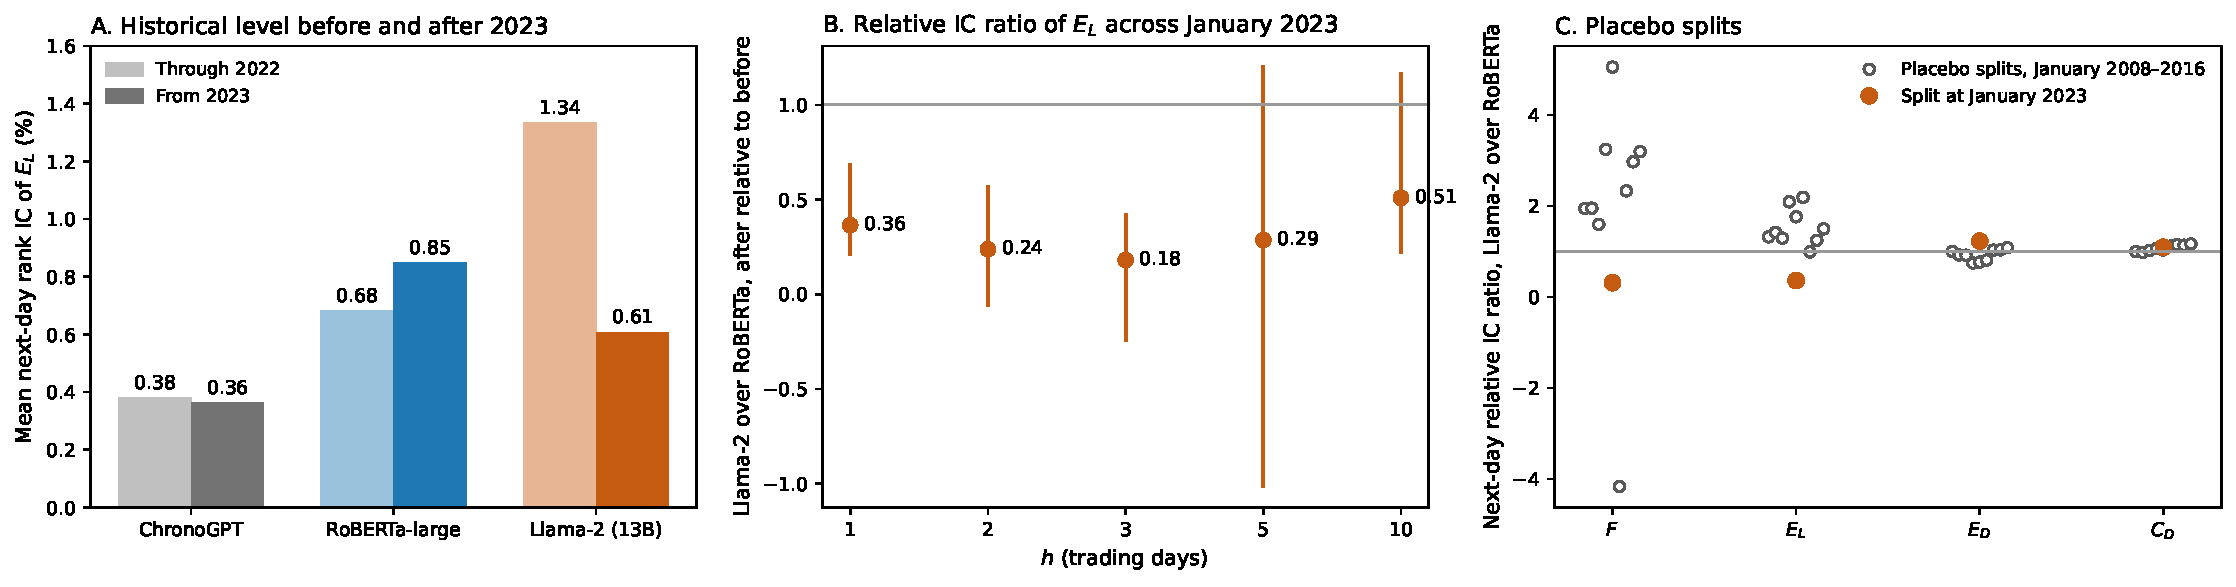
\includegraphics[width=\textwidth]{cal_cutoff_ic.pdf}
\begin{minipage}{\linewidth}\footnotesize
This figure reports historical-level rank ICs and relative IC ratios on common trading days. Panel A gives the historical level's mean next-day rank IC before and after January 2023 for ChronoGPT$_{1999}$, RoBERTa-large, and Llama-2 (13B). Panel B gives Llama-2's historical-level relative IC ratio against RoBERTa across January 2023 at horizon $h$ trading days, with 90\% intervals from 40-day moving blocks drawn within periods. Panel C gives next-day relative IC ratios for firm identity $F$, the historical level $E_L$, the deviation $E_D$, and category deviation $C_D$, at a split each January from 2008 to 2016 (hollow) and across January 2023 (filled). Each placebo sample runs from 2004 through three years after the split. Relative IC ratios divide Llama-2's after-to-before IC ratio by RoBERTa's.
\end{minipage}
\end{figure}

\paragraph{Full-forecast comparisons.}
CKX compare portfolio performance across an encoder's pretraining cutoff, while DKPT compare strategy performance across ChronoGPT vintages.\footnote{Didisheim et al. (2026) and Kelly et al. (2026) find similar strategy Sharpe ratios for point-in-time and full-sample versions of their models. In our framework, the effect of later pretraining depends on an encoder's ability to extract persistent firm information and its loading on memory. These effects can differ across models, particularly as representation capacity changes.}
Such comparisons may obscure look-ahead bias concentrated in the historical level.

For the representative firm above, memory enters the historical level. Let $\Gamma$ denote total predictive covariance and $\Delta\Gamma$ its change attributable to memory, holding other sources of predictability fixed. Since $\Delta\Gamma=\Delta\Gamma_{E_L}$,
\begin{equation}\label{eq:D30}
\frac{\Delta\Gamma}{\Gamma}
=\frac{\Gamma_{E_L}}{\Gamma}
\frac{\Delta\Gamma_{E_L}}{\Gamma_{E_L}}.
\end{equation}
The effect on full-forecast predictability is therefore scaled by the historical level's share of total predictive covariance. This share is small for CKX's next-day forecasts, where category deviations dominate. For DKPT's MSRR strategy, changes in Sharpe ratios also depend on portfolio optimization and return volatility, so they need not track changes in historical-level predictability. Component-level comparisons thus provide a more direct assessment of look-ahead bias.

\paragraph{Lagged historical level.}
We next consider how the predictive performance of the historical level changes when measured 36 months earlier. Under stationarity and comparable news coverage, the lagged and current levels have the same variance, while the lagged level's covariance with future state premia is reduced by the factor
\begin{equation}\label{eq:D31}
\frac{\Var(\bar z)+\bar\rho_L\rho_m^{36}\Var(x)}
{\Var(\bar z)+\bar\rho_L\Var(x)}.
\end{equation}
The permanent state remains informative, while the evolving state's contribution decays with $\rho_m^{36}$. In the data, the lagged level is available for 83\% as many firm-months as the current-level signal.\footnote{The ratio is computed among firm-months with news and next-month returns. Lagged coverage requires news during months $\tau-48$ through $\tau-37$, while current-level coverage requires either an estimated firm effect or news during months $\tau-12$ through $\tau-1$.}
By \eqref{eq:D16}, the Sharpe ratio without memory is therefore approximately $\sqrt{0.83}$ times \eqref{eq:D31} times that of the current-level strategy, assuming comparable signal quality across the two samples.

Memory, unlike the evolving state, is constant across a firm's news items and does not decay when the historical level is lagged. Lagging therefore reduces the historical level's state-related predictability without similarly reducing its memory-related predictability. Under the reoptimized MSRR weights in \eqref{eq:D15}, each independent predictive direction contributes to expected strategy returns in proportion to its squared covariance with returns divided by its variance. Holding signal variances fixed, the state contribution relative to memory declines by the square of the factor in \eqref{eq:D31}.

\section{Calibration}\label{sec:calibration}

Returns around news announcements inform event drift, while the distribution of predictability across components and horizons informs the persistence and measurement of firm information. Changes in predictability around pretraining cutoffs help distinguish persistent firm information from memory. The calibration proceeds in two steps: preliminary parameter calibration followed by a joint search for the remaining parameters.

\paragraph{Preliminary calibration.}
Panel A of Table~\ref{tab:D2} reports the parameters fixed before the joint search. We determine $\kappa$ and $\vartheta$ from the category long--short portfolio's announcement-day return and its cumulative returns from the first eligible open through trading days 1 and 10. Up to the portfolio's return per unit of signal, these correspond to the two terms of \eqref{eq:D1}. The calibrated values are $\kappa=0.68$ and $\vartheta=0.26$, so about 98\% of post-announcement drift is complete by trading day three.

We set $\Var(m_K)$ using the category-mean forecast's next-day predictive covariance, $\delta_1^2\Var(m_K)$. A forecast's long--short return is proportional to its covariance with returns divided by its standard deviation, while its raw Fama--MacBeth slope is the covariance divided by its variance. Thus, the squared long--short return divided by the slope is proportional to predictive covariance, with a common proportionality constant for forecasts evaluated on the same firm-days. We use this relation to infer the category-mean covariance from each embedding forecast's covariance and average the estimates from RoBERTa and Llama-2.

For Llama-2, we set $\phi(q)$ so that \eqref{eq:D7} equals its out-of-sample SUE $R^2$ gain of 3.2 percentage points, with event categories explaining 1.9\% of SUE variation. The out-of-sample gain lies below its population counterpart by Proposition~\ref{prop:D1}. Daily moments identify only $\phi(g)\pi^2$, so we fix Llama-2's state loading at $g=1$. The memory window follows Crane et al. (2025), while the news-count parameters are measured directly from the data. In \eqref{eq:D8}, we set $\sigma_r$ so that RoBERTa's model IC equals its data IC.

\begin{table}[htbp]
\centering
\caption{Calibrated Parameters}
\label{tab:D2}
\begin{minipage}{\linewidth}\footnotesize
This table reports the calibrated parameters for ChronoGPT$_{1999}$, RoBERTa-large and Llama-2 (13B). Panel A lists values set before the joint search, Panel B the values from the search, and Panel C quantities implied by them. Source gives the moments or equations that mainly determine each value. The category signal and the story detail are in percent of value, and the state premium is in basis points per trading day. $\Upsilon$ converts monthly covariances times $10^6$ into percent per year. The levels of $\phi(g)$ and $\pi$ are conditional on fixing Llama-2's $g$ at one. The last two rows are averages over the strategies' signal months, including those after each encoder's pretraining cutoff.
\end{minipage}
\medskip

{\footnotesize
\begin{adjustbox}{max width=\linewidth}
\begin{tabular}{llccccl}
\toprule
Parameter & Description & Common & ChronoGPT$_{1999}$ & RoBERTa & Llama-2 & Source \\
\midrule
\multicolumn{7}{@{}l}{\textit{Panel A: Set before the search}} \\
$\kappa$ & Announcement response & 0.68 &  &  &  & Category long--short return, \eqref{eq:D1} \\
$\vartheta$ & Daily drift decay & 0.26 &  &  &  & Category long--short return, \eqref{eq:D1} \\
$\mathrm{sd}(m_K)$ & Category signal & 0.52 &  &  &  & Category-mean long--short return and slope \\
$q$ & Detail loading &  &  &  & 0.18 & SUE $R^2$ gain, \eqref{eq:D7} \\
$g$ & State loading &  &  &  & 1 & Normalization \\
$N_\theta$ & Memory window, months &  &  & 360 & 360 & Crane et al. (2025) \\
$\bar n$ & News items per firm-month & 3.86 &  &  &  & Harmonic mean in the data \\
$\bar n^F$ & News items per firm, valuation windows & 189 &  &  &  & Data, \eqref{eq:D20} \\
\midrule
\multicolumn{7}{@{}l}{\textit{Panel B: Joint search}} \\
$\mathrm{sd}(\nu)$ & Detail & 1.06 &  &  &  & Daily $I_D$, \eqref{eq:D34} \\
$\pi$ & State premium & 2.7 &  &  &  & Daily $F$ net of memory, \eqref{eq:D32} \\
$\Var(\bar z)$ & Permanent share & 0.29 &  &  &  & $F$, $I_L$, \eqref{eq:D32}--\eqref{eq:D36} \\
$\rho_m$ & Monthly state persistence & 0.983 &  &  &  & Monthly components, \eqref{eq:D35}--\eqref{eq:D37} \\
$a$ & Category-signal loading &  & 0.88 & 0.95 & 1.03 & Daily $C_D$, \eqref{eq:D2} \\
$q$ & Detail loading &  & 0.14 & 0.14 &  & Daily $I_D$, \eqref{eq:D34} \\
$g$ & State loading &  & 0.39 & 0.43 &  & Daily $F$, $I_L$, monthly components \\
$\eta$ & Memory loading &  &  & 0.12 & 2.20 & IC ratios (Llama-2), monthly $F$, $I_L$ (RoBERTa) \\
$\Upsilon$ & Monthly strategy scale &  & 1.47 & 6.39 & 6.12 & Monthly components, \eqref{eq:D17} \\
$\sigma_\theta^2$ & Cash-flow-news variance, monthly & 0.011 &  &  &  & \eqref{eq:D23}, jointly with $\pi$ \\
\midrule
\multicolumn{7}{@{}l}{\textit{Panel C: Implied}} \\
 & Half-life of $x$, months & 39 &  &  &  & $\ln 2/(-\ln\rho_m)$ \\
$\phi(g)$ & Reliability of the state measure &  & 0.13 & 0.16 & 0.50 & $g^2/(1+g^2)$ \\
$\phi(\eta)$ & Reliability of the memory measure &  &  & 0.01 & 0.83 & $\eta^2/(1+\eta^2)$ \\
 & Memory's share of the first-month mean return, MSRR on $E_L$ (\%) &  & 0 & 24 & 47 & \eqref{eq:D16}, \eqref{eq:D26} \\
 & Memory's share of the first-month mean return, MSRR on $E_{L,\tau-36}$ (\%) &  & 0 & 40 & 66 & \eqref{eq:D16}, \eqref{eq:D31} \\
\bottomrule
\end{tabular}
\end{adjustbox}
}
\end{table}

\paragraph{Coverage shares.}
The model in Section~\ref{sec:param} describes a representative firm with news throughout the projection window, whereas the empirical decomposition retains all firms in the CKX and DKPT samples, including those with short news histories. For a firm covered only in the final year of the projection window, $\bar x^F$ and $\bar x^L$ would reflect similar news periods, causing $F$ to capture recent information rather than long-run firm information. To maintain a comparable interpretation of $F$ across firms, Section~\ref{sec:decomp} sets $F$ to zero for firms with fewer than ten news items in the projection window or news in only one calendar year, without excluding these firms from the sample.

For firms with $F=0$, persistent firm information that would otherwise enter $F$, including the permanent state, $\bar x^F$, and memory, instead enters $I_L$ if the firm has news in the preceding 12 months and $I_D$ otherwise. The remaining historical variation in the evolving state, $\bar x^L-\bar x^F$, likewise enters $I_L$ when trailing news is available and $I_D$ otherwise. Table~\ref{tab:D3} reports the shares $\varpi_F$, $\varpi_{I_L}$, and $\varpi_{I_D}$ associated with these assignments, together with the share $H$ of observations with news in the preceding 12 months.\footnote{Firm effects are determined from each test year's two-way projection. Shares are computed over firm-days for daily forecasts and over firm-months with news and next-month returns for monthly strategies, averaging news items within each firm-day or firm-month.} Assuming comparable average predictive covariance per observation across the three groups, these shares allocate persistent firm information's pooled covariance across $F$, $I_L$, and $I_D$. The shares are measured in the data, not calibrated.

\begin{table}[htbp]
\centering
\caption{Coverage Shares and Component Assignment}
\label{tab:D3}
\begin{minipage}{\linewidth}\footnotesize
This table reports the shares of firm-days and firm-months by whether the firm effect is estimated and whether the observation has a historical level. Component is where persistent firm information enters, and $H$ is the share of observations with news in the preceding 12 months.
\end{minipage}
\medskip

{\footnotesize
\begin{adjustbox}{max width=\linewidth}
\begin{tabular}{lcccc}
\toprule
 & Share & Component & Firm-days & Firm-months \\
\midrule
Firm effect estimated & $\varpi_F$ & $F$ & 0.936 & 0.912 \\
$F=0$, historical level available & $\varpi_{I_L}$ & $I_L$ & 0.061 & 0.081 \\
$F=0$, no historical level & $\varpi_{I_D}$ & $I_D$ & 0.003 & 0.007 \\
News available in the preceding 12 months & $H$ & & 0.996 & 0.991 \\
\bottomrule
\end{tabular}
\end{adjustbox}
}
\end{table}

Using the firm-day coverage shares in Table~\ref{tab:D3}, the daily predictive covariances of $F$, $I_L$, and $I_D$, including memory, which are the model values for the daily targets of the joint search, are
\begin{equation}\label{eq:D32}
\Gamma_{F,t}(h) = \varpi_F\left[\phi(g)\pi^2\left(\Var(\bar z)+\bar\rho_F\rho^{h-1}\Var(x)\right)+M_t(h)\right]
\end{equation}
\begin{equation}\label{eq:D33}
\begin{split}
\Gamma_{I_L,t}(h) &= \varpi_{I_L}\left[\phi(g)\pi^2\left(\Var(\bar z)+\bar\rho_F\rho^{h-1}\Var(x)\right)+M_t(h)\right]\\
&\quad + H\phi(g)\pi^2(\bar\rho_L-\bar\rho_F)\rho^{h-1}\Var(x)
\end{split}
\end{equation}
\begin{equation}\label{eq:D34}
\begin{split}
\Gamma_{I_D,t}(h) &= \phi(q)\delta_1\delta_h\Var(\nu) + \varpi_{I_D}\left[\phi(g)\pi^2\left(\Var(\bar z)+\bar\rho_F\rho^{h-1}\Var(x)\right)+M_t(h)\right]\\
&\quad + \phi(g)\pi^2\left((1-H)(\bar\rho_L-\bar\rho_F)+1-\bar\rho_L\right)\rho^{h-1}\Var(x)
\end{split}
\end{equation}
Let $M^m_\tau(h)$ equal \eqref{eq:D26} for a remembered return month and zero otherwise. Using the firm-month coverage shares, the monthly predictive covariances, which give the model values for the monthly targets up to the scale $\Upsilon$, are
\begin{equation}\label{eq:D35}
\Gamma^m_{F,\tau}(h) = \varpi_F\left[\phi(\sqrt{\bar n}g)\pi_m^2\left(\Var(\bar z)+\bar\rho_F\rho_m^{h-1}\Var(x)\right)+M^m_\tau(h)\right]
\end{equation}
\begin{equation}\label{eq:D36}
\begin{split}
\Gamma^m_{I_L,\tau}(h) &= \varpi_{I_L}\left[\phi(\sqrt{\bar n}g)\pi_m^2\left(\Var(\bar z)+\bar\rho_F\rho_m^{h-1}\Var(x)\right)+M^m_\tau(h)\right]\\
&\quad + H\phi(\sqrt{\bar n}g)\pi_m^2(\bar\rho_L-\bar\rho_F)\rho_m^{h-1}\Var(x)
\end{split}
\end{equation}
\begin{equation}\label{eq:D37}
\begin{split}
\Gamma^m_{I_D,\tau}(h) &= \bar n\phi(q)\bar\delta_1\bar\delta_h\Var(\nu) + \varpi_{I_D}\left[\phi(\sqrt{\bar n}g)\pi_m^2\left(\Var(\bar z)+\bar\rho_F\rho_m^{h-1}\Var(x)\right)+M^m_\tau(h)\right]\\
&\quad + \phi(\sqrt{\bar n}g)\pi_m^2\left((1-H)(\bar\rho_L-\bar\rho_F)+1-\bar\rho_L\right)\rho_m^{h-1}\Var(x)
\end{split}
\end{equation}
The memory covariances $\bar M_{j,p}^o$ in \eqref{eq:D27}--\eqref{eq:D29} correspond to the period averages of the memory terms in \eqref{eq:D32}--\eqref{eq:D34}.

Although news from firms assigned $F=0$ accounts for only a small share of observations, their persistent firm information enters $I_L$ when historical news is available. Because, in the data, $I_L$'s predictive covariance is less than half that of $F$, this information can account for a sizeable share of $I_L$'s predictability. The permanent state of these firms can thus help explain the persistence of $I_L$'s returns across months.

\paragraph{Joint search.}
The second step minimizes
\[
\sum_{\mathcal B}\frac{1}{|\mathcal B|}\sum_{j\in\mathcal B}
\left(\frac{\hat m_j-m_j}{\mathrm{se}(\hat m_j)}\right)^2,
\]
where $\hat m_j$ is an empirical moment, $m_j$ its model counterpart, and $\mathrm{se}(\hat m_j)$ its standard error. The search chooses 16 parameters, with $\sigma_\theta^2$ solved jointly, to match the 49 moments of Table~\ref{tab:D4} below its first row. Each block $\mathcal B$ receives equal weight, regardless of the number of moments it contains. Each block contains one decomposition component's moments at one frequency, across encoders and targeted horizon bands. Each cutoff comparison's relative next-day IC ratios of $F$ and $E_L$ form a further block. For equal standardized discrepancies, each relative IC ratio weighs 9/2 times a monthly moment, because its block has two moments and a monthly block nine.

We use diagonal standard-error weights rather than estimating the full covariance matrix of the moments. Sampling errors in that matrix can be correlated with sampling errors in the moments, producing small-sample bias in optimally weighted minimum-distance estimates (Altonji and Segal, 1996). Band standard errors are Newey--West, with five daily or six monthly lags plus the band's width minus one. For relative IC ratios, we infer standard errors from their 90\% confidence intervals under a normal approximation.

The cash-flow-news variance is determined by \eqref{eq:D23} within the joint search. The variance of 36-month returns is 0.415, estimated from seven non-overlapping windows starting in January 2004.\footnote{Winsorization is at 1\% and 99\%. The sample is firms with news in the calendar year and returns in all 36 months of the window.}
The state-premium variance depends on $\pi$, $\Var(\bar z)$, and $\rho_m$, so \eqref{eq:D23} is a constraint solved jointly with these parameters, not a targeted moment. At the calibrated parameters, state premia account for about 9\% of the 36-month return variance, yielding $\sigma_\theta^2=0.011$. Without subtracting the state-premium variance, the monthly variance would be 0.0115. All 64 scrambled Sobol starts over wide parameter ranges reach the reported minimum.

\begin{table}[htbp]
\centering
\caption{Targeted Moments and Fit}
\label{tab:D4}
\begin{minipage}{\linewidth}\footnotesize
This table reports the moments targeted in the joint search, for ChronoGPT$_{1999}$, RoBERTa-large and Llama-2 (13B). Strategy returns are the residualized-embedding strategy's fixed-weight component returns before any horizon-specific volatility scaling, which by Proposition~\ref{prop:D2} equal $\Upsilon$ times the model's monthly covariances. Horizon bands are averages. Equation gives the model value. RMS $t$ is the root mean squared ratio of the data-minus-model difference to the standard error over the block's moments. The first row is matched exactly before the joint search.
\end{minipage}
\medskip

{\footnotesize
\begin{adjustbox}{max width=\linewidth}
\begin{tabular}{lcccc}
\toprule
Moment & Equation & Horizons & Count & RMS $t$ \\
\midrule
Cumulative category long--short return & \eqref{eq:D1} & Days 0, 1, 10 & 3 & 0.00 \\
\multicolumn{5}{@{}l}{\textit{Daily covariance with returns}} \\
$C_D$ & \eqref{eq:D2} & Day 1; days 2--10 & 6 & 0.71 \\
$I_D$ & \eqref{eq:D34} & Day 1; days 2--10 & 6 & 0.98 \\
$F$ & \eqref{eq:D32} & Days 2--10 & 3 & 0.73 \\
$I_L$ & \eqref{eq:D33} & Days 2--10 & 3 & 0.68 \\
\multicolumn{5}{@{}l}{\textit{MSRR strategy return}} \\
$F$ & \eqref{eq:D35} & Months 2--12, 13--24, 25--36 & 9 & 0.71 \\
$I_L$ & \eqref{eq:D36} & Months 2--12, 13--24, 25--36 & 9 & 1.14 \\
$I_D$ & \eqref{eq:D37} & Months 2--12, 13--24, 25--36 & 9 & 0.58 \\
\multicolumn{5}{@{}l}{\textit{Relative IC ratios of $F$ and $E_L$}} \\
Llama-2, January 2023 & \eqref{eq:D28} & Next day & 2 & 0.23 \\
RoBERTa, January 2020 & \eqref{eq:D29} & Next day & 2 & 0.26 \\
\midrule
Sobol starts reaching the minimum & & & 64 of 64 & \\
\bottomrule
\end{tabular}
\end{adjustbox}
}
\end{table}



\paragraph{Calibration targets and identification.}
We target the first horizon only where the model attributes predictability to event drift, namely daily $C_D$ and $I_D$. State-related daily targets and all monthly targets begin at horizon 2, except the relative IC ratios, which use next-day rank ICs and, unlike covariances, show no day-one excess. Little event drift remains after the signal month, so the monthly targets primarily identify state persistence, the permanent share, and the allocation of predictability across components.



Day-one $C_D$ determines the category-signal loading $a$. Given Llama-2's $\phi(q)$, its day-one $I_D$ determines $\Var(\nu)$, while the other encoders' day-one $I_D$ determines their $q$. The decay of monthly returns across horizon bands and the split between $F$ and $I_L$ determine $\rho_m$ and the permanent share. Llama-2's memory loading is primarily determined by its relative IC ratios. RoBERTa's memory loading balances its monthly $F$, which favors more memory, against the relative IC ratios from both cutoff comparisons and its monthly $I_L$, which constrain it.

The state premium connects the cutoff comparisons to the other calibration targets. With Llama-2's $g=1$, $\pi$ is primarily determined by its daily $F$ covariance net of memory, while the relative IC ratios determine the memory share of that covariance. The state premium also enters the return-variance restriction in \eqref{eq:D23}. Llama-2's $\phi(\eta)=0.83$ places its memory covariance at 83\% of the bound in Section~\ref{sec:lookahead}, so extending the memory window would leave less room for memory to match the cutoff ratios.

The monthly calibration involves two approximations. First, each encoder's strategy has a single scale $\Upsilon$, defined in \eqref{eq:D17}, which absorbs the overall scale of MSRR shrinkage. Because ridge shrinkage varies across predictive directions, using one $\Upsilon$ for all components and horizons is an approximation. The monthly targets therefore constrain the other parameters through relative component magnitudes and term structures. Second, monthly model values assume that the characteristics are uncorrelated with the permanent state and with current and past values of the evolving state, so that $z_X^j=0$ for each component and \eqref{eq:D18} reduces to \eqref{eq:D11}--\eqref{eq:D13}. Residualization leaves $\rho_m$ unchanged for any $X$, so the decay of monthly predictability still identifies state persistence. The calibrated permanent share and allocation across components, however, depend on this assumption.

The excluded first-horizon moments provide checks on the model. In the data, firm identity's day-one covariance is about two to three times its average over days 2--10 for all three encoders, including ChronoGPT, whereas its rank IC is nearly unchanged: 0.23\% versus 0.26\% for ChronoGPT, 0.47\% versus 0.47\% for RoBERTa, and 1.09\% versus 1.02\% for Llama-2. This suggests that the excess day-one covariance reflects differences in return magnitudes or tails rather than stronger rank predictability. The model's state component, whose covariance changes little across days, does not capture this pattern.

Monthly $I_D$ also exhibits a pronounced first-horizon difference. Its month-one return exceeds its month-two return for all three encoders. For RoBERTa, the return standard deviation is similar across months 1, 2, and 3, indicating that the difference is primarily in mean returns. Refitting MSRR weights to month-two returns raises $I_D$'s annualized month-two return before volatility scaling from 2.3\% to 32.6\% for RoBERTa and from 20.9\% to 57.3\% for Llama-2, while RoBERTa's firm identity changes little, from 83.3\% to 79.9\%.
For ChronoGPT, the corresponding $I_D$ return rises from 0.9\% to 7.5\%.
Thus, weights fitted to month-one returns capture substantially less of the deviation's predictive content in month two than weights fitted to month-two returns. The calibrated model, with little event drift beyond the signal month and a single direction for the persistent state, cannot account for the magnitude of this horizon dependence.

\paragraph{Alternative specifications.}
Table~\ref{tab:D5} examines the sensitivity of the calibrated outcome-memory shares and state persistence to alternative specifications. We exclude discount-rate news from the variance available to memory,\footnote{About 18\% of $\sigma_\theta^2$ represents discount-rate news rather than cash-flow news. Since memory covariance depends on $\sigma_\theta^2/N_\theta$, excluding this portion is equivalent to extending the memory window from 30 to about 37 years.} include month-one $F$ and $I_L$ returns among the targets, and set $\varpi_F=1$ instead of using the empirical coverage shares. We also allow observed characteristics to explain part of the state,\footnote{We set $R^2(z\mid X)=0.29$, the valuation $R^2$ implied by \eqref{eq:D20} for RoBERTa. We do not use Llama-2's 0.47, which may reflect remembered valuations. At the baseline loadings, this assumption implies that characteristics explain about 12\% of RoBERTa's and 23\% of Llama-2's variance along the monthly state coordinate.} impose $\Var(\bar z)=0$, or allow separate monthly scales $\Upsilon$ for $F$ and $I_L$.

Llama-2's outcome-memory shares remain between 67\% and 76\% for $F$ and between 61\% and 66\% for $E_L$, constrained by the same relative IC ratios targeted in every specification. RoBERTa's corresponding shares range from zero to 31\% and from zero to 22\%, respectively, remaining below half of Llama-2's in every specification. Excluding discount-rate news pushes Llama-2's memory reliability $\phi(\eta)$ to its upper bound, as less variance available for memory requires a more reliable memory measure to match the cutoff ratios.

Long-horizon state persistence is also relatively stable. The firm state's 36-month autocorrelation ranges from 0.58 to 0.71, compared with 0.67 in the baseline, even as the evolving state's half-life varies from 11 to 67 months. In particular, setting $\Var(\bar z)=0$ still produces a 36-month autocorrelation of 0.69, with a half-life of 67 months. The separate-scale specification yields a similar autocorrelation but has multiple local minima, with only 38 of 64 starts reaching the reported minimum. Thus, the calibration consistently implies persistent firm information, although its division between permanent and evolving states is sensitive to the specification.

\begin{table}[htbp]
\centering
\caption{Calibration under Alternative Specifications}
\label{tab:D5}
\begin{minipage}{\linewidth}\footnotesize
This table reports the joint search under alternative specifications. Memory share is the percentage of the component's next-day predictive covariance attributable to memory, $1-\omega_j^o$, before January 2023 for Llama-2 and January 2020 for RoBERTa. $\rho_z(36)=\Var(\bar z)+\rho_m^{36}\Var(x)$ is the autocorrelation of the firm state at 36 months, the longest horizon of the monthly targets. Loss is the minimized criterion of the joint search. Each search runs from 64 starting values.
\end{minipage}
\medskip

{\footnotesize
\begin{adjustbox}{max width=\linewidth}
\begin{tabular}{lccccccccc}
\toprule
 & \multicolumn{2}{c}{Llama-2 memory (\%)} & \multicolumn{2}{c}{RoBERTa memory (\%)} & Llama-2 & Half-life of $x$ & & & Convergence to \\
\cmidrule(lr){2-3}\cmidrule(lr){4-5}
Specification & $F$ & $E_L$ & $F$ & $E_L$ & $\phi(\eta)$ & (months) & $\rho_z(36)$ & Loss & same minimum \\
\midrule
Baseline & 70 & 62 & 11 & 8 & 0.83 & 39 & 0.67 & 4.72 & 64/64 \\
$0.82\,\sigma_\theta^2$ in memory & 69 & 62 & 9 & 7 & 1.00 & 39 & 0.68 & 4.54 & 64/64 \\
$h=1$ targeted for $F$ and $I_L$ & 69 & 61 & 9 & 7 & 0.83 & 36 & 0.67 & 5.17 & 64/64 \\
$\varpi_F=1$ & 72 & 61 & 21 & 14 & 0.88 & 45 & 0.58 & 5.56 & 64/64 \\
$R^2(z\mid X)=0.29$ & 76 & 66 & 31 & 22 & 0.89 & 47 & 0.60 & 5.32 & 64/64 \\
$\Var(\bar z)=0$ & 72 & 64 & 18 & 13 & 0.86 & 67 & 0.69 & 4.80 & 64/64 \\
Separate $\Upsilon$ for $F$ and $I_L$ & 67 & 62 & 0 & 0 & 0.81 & 11 & 0.71 & 3.05 & 38/64 \\
\bottomrule
\end{tabular}
\end{adjustbox}
}
\end{table}

\section{Model Values against the Data}\label{sec:modeldata}

\subsection{Untargeted Moments}

Table~\ref{tab:tab13} reports model values outside the calibration targets in two groups. The upper panel contains statistics whose levels are not pinned by targeted moments. The lower panel contains values that follow from targeted moments through the model's restrictions. These comparisons assess the magnitudes of the mechanisms in Sections~\ref{sec:param} and~\ref{sec:lookahead}, using the parameters of Section~\ref{sec:calibration}.

The monthly-averaged daily forecast is the headline-weighted monthly average of a firm's daily forecasts. No moment of this forecast enters the calibration, and its components have no free scale. Its month-one $F+I_L$ covariance, multiplied by $10^6$, is 0.23 in the model against 0.57 in the data for RoBERTa and 1.67 against 2.02 for Llama-2. Its covariance also decays more slowly in the model.

By \eqref{eq:D20}, the ratio of Llama-2's to RoBERTa's valuation $R^2$ from the model's state is 1.03, below the data's ratio of 1.67. Firm identity averages about 189 news items, so language noise largely averages out, and the state accounts for a similar share of both encoders' firm-identity variance. This calculation excludes the possibility that embeddings contain memory of information already reflected in valuations, which may contribute to the difference.

The model's SUE $R^2$ gain for RoBERTa is 1.8 percentage points, against 0.8 in the data. The model value is a population gain, whereas the data value is out of sample. Proposition~\ref{prop:D1} shows how estimation noise reduces the out-of-sample gain. Llama-2's gain is matched by construction and therefore provides no separate check.

\begin{table}[htbp]
\centering
\caption{Model and Data Statistics outside the Targets}
\label{tab:tab13}
\begin{minipage}{\linewidth}\footnotesize
This table reports model and data values of statistics that the calibration does not target, for RoBERTa-large and Llama-2 (13B). No targeted moment pins the upper panel's model values, while the lower panel's follow from targeted moments through the model's structure. Model values include memory, and the IC and Mincer--Zarnowitz rows approximate the forecast's variance along the memory direction by the mean memory component of its covariance with returns. The monthly-averaged daily forecast is the headline-weighted monthly average of a firm's daily ridge forecasts. $F+I_L$ is firm identity plus the idiosyncratic historical level. The month-1 $F+I_L$ and day-one rows are covariances with returns, multiplied by $10^6$. The lagged level is the historical level 36 months earlier, and valuation is log price-to-book. Model SUE gains are population values and data gains out of sample, while model ICs are Pearson and data ICs rank correlations on firm-days with returns over the ten subsequent trading days. Norm.\ marks values matched by construction.
\end{minipage}
\medskip

{\footnotesize
\begin{adjustbox}{max width=\linewidth}
\begin{tabular}{lccccl}
\toprule
 & \multicolumn{2}{c}{Model} & \multicolumn{2}{c}{Data} & \\
\cmidrule(lr){2-3}\cmidrule(lr){4-5}
Statistic & RoBERTa & Llama-2 & RoBERTa & Llama-2 & Equation \\
\midrule
\multicolumn{6}{@{}l}{\textit{Levels outside the targets}} \\
Monthly-averaged daily forecast, $F+I_L$, month 1 & 0.23 & 1.67 & 0.57 & 2.02 & \eqref{eq:D14}, \eqref{eq:D26} \\
Lagged historical level, month-1 Sharpe ratio over the current level's & 0.68 & 0.76 & 0.27 & 0.56 & \eqref{eq:D16}, \eqref{eq:D31} \\
SUE $R^2$ gain from the embedding (pp) & 1.8 & norm. & 0.8 & 3.2 & \eqref{eq:D7} \\
Firm-identity valuation $R^2$ from the state, Llama-2 over RoBERTa & \multicolumn{2}{c}{1.03} & \multicolumn{2}{c}{1.67} & \eqref{eq:D20} \\
\midrule
\multicolumn{6}{@{}l}{\textit{Model restrictions}} \\
Firm identity, day one & 0.007 & 0.066 & 0.057 & 0.189 & \eqref{eq:D32} \\
Monthly-averaged daily forecast, $F+I_L$, month 12 over month 1 & 0.89 & 0.95 & 0.33 & 0.82 & \eqref{eq:D14}, \eqref{eq:D26} \\
MSRR strategy, historical-level share, month 1 (\%) & 92.1 & 95.3 & 51.0 & 76.3 & \eqref{eq:D10}, \eqref{eq:D35}--\eqref{eq:D37} \\
Mincer--Zarnowitz slope & 0.86 & 0.89 & 0.70 & 0.66 & \eqref{eq:D9} \\
Embedding forecast IC (\%) & norm. & 2.73 & 2.41 & 2.66 & \eqref{eq:D8} \\
\bottomrule
\end{tabular}
\end{adjustbox}
}
\end{table}

\subsection{Trading-Day Horizons}

Event drift fades within days, while the state's contribution to expected returns changes little from day to day. The category deviation accounts for most predictive covariance at the shortest horizons in Figure~\ref{fig:pf2a}.
The model's historical-level covariance exceeds the category deviation's at about 4.1 trading days for RoBERTa and 2.7 for Llama-2. Llama-2's larger state loading and memory raise its level, and the level exceeds the full deviation's shortly afterward.

\begin{figure}[!htbp]
\centering
\caption{Daily Forecast Covariances by Component and Horizon}
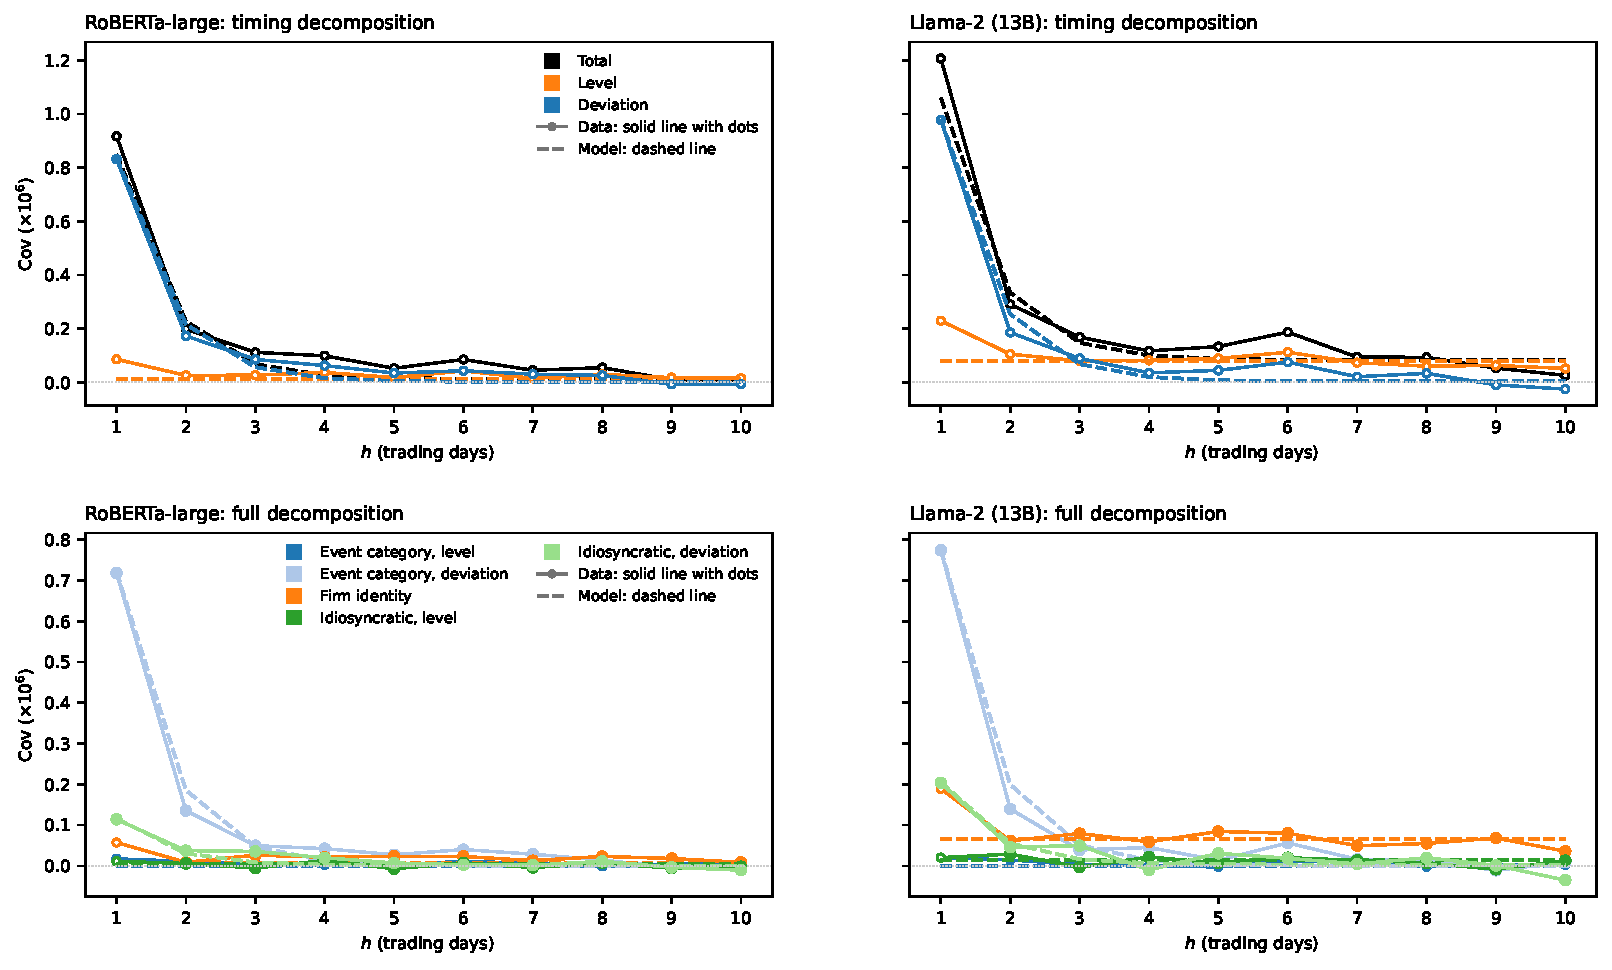
\includegraphics[width=\linewidth]{cal_fig2a.pdf}
\label{fig:pf2a}
\begin{minipage}{\linewidth}\footnotesize
This figure reports daily forecast covariances with returns $h$ trading days after news. Columns show RoBERTa-large and Llama-2 (13B), with the timing decomposition (total, historical level, deviation) in the upper panels and the full decomposition ($C_L$, $C_D$, $F$, $I_L$, $I_D$) in the lower panels. Data are solid lines with dots, targeted horizons have filled markers, and model values are dashed lines. Model category-level covariance is zero.
\end{minipage}
\end{figure}

Because event drift dominates next-day predictability, Llama-2's larger state loading adds little to daily IC. Setting the daily return standard deviation $\sigma_r$ to match RoBERTa's IC gives a Llama-2 IC of 2.73\%, including memory, compared with 2.66\% in the data. This model value follows largely from the day-one targets once $\sigma_r$ is set. Model ICs are Pearson correlations, while data ICs are rank correlations.

The ridge fits have about 153 effective parameters for RoBERTa and 154 for Llama-2. Proposition~\ref{prop:D1} maps estimation noise into lower ICs and Mincer--Zarnowitz slopes. The model slopes are 0.86 and 0.89, against 0.70 and 0.66 in the data, so estimation noise explains only part of the slopes' shortfall below one.

The category-mean forecast avoids the embedding's imperfect measurement of the category signal, and \eqref{eq:D6} gives the condition under which its next-day $R^2$ exceeds the embedding forecast's.
Ridge forecasts estimated on category centroids have empirical ICs of 3.15\% for RoBERTa and 3.14\% for Llama-2, compared with embedding ICs of 2.41\% and 2.66\%.

\subsection{Monthly Averaging and the Monthly Projection Forecast}

Little event drift remains after the signal month (6.4\% of post-announcement drift in the first following month). The state premium accrues over every trading day of the return month. Monthly averaging therefore concentrates the model's predictive covariance in the historical level, whose covariance declines slowly with the horizon. Figure~\ref{fig:pf2b} compares the monthly-averaged daily forecast with the model. By month 12, the model retains 89\% of its month-one $F+I_L$ covariance for RoBERTa and 95\% for Llama-2, against 33\% and 82\% in the data. The model has one persistence for all encoders. RoBERTa's and ChronoGPT's firm information decays faster than this persistence implies.

\begin{figure}[!htbp]
\centering
\caption{Monthly-Averaged Daily Forecast Covariances by Component and Horizon}
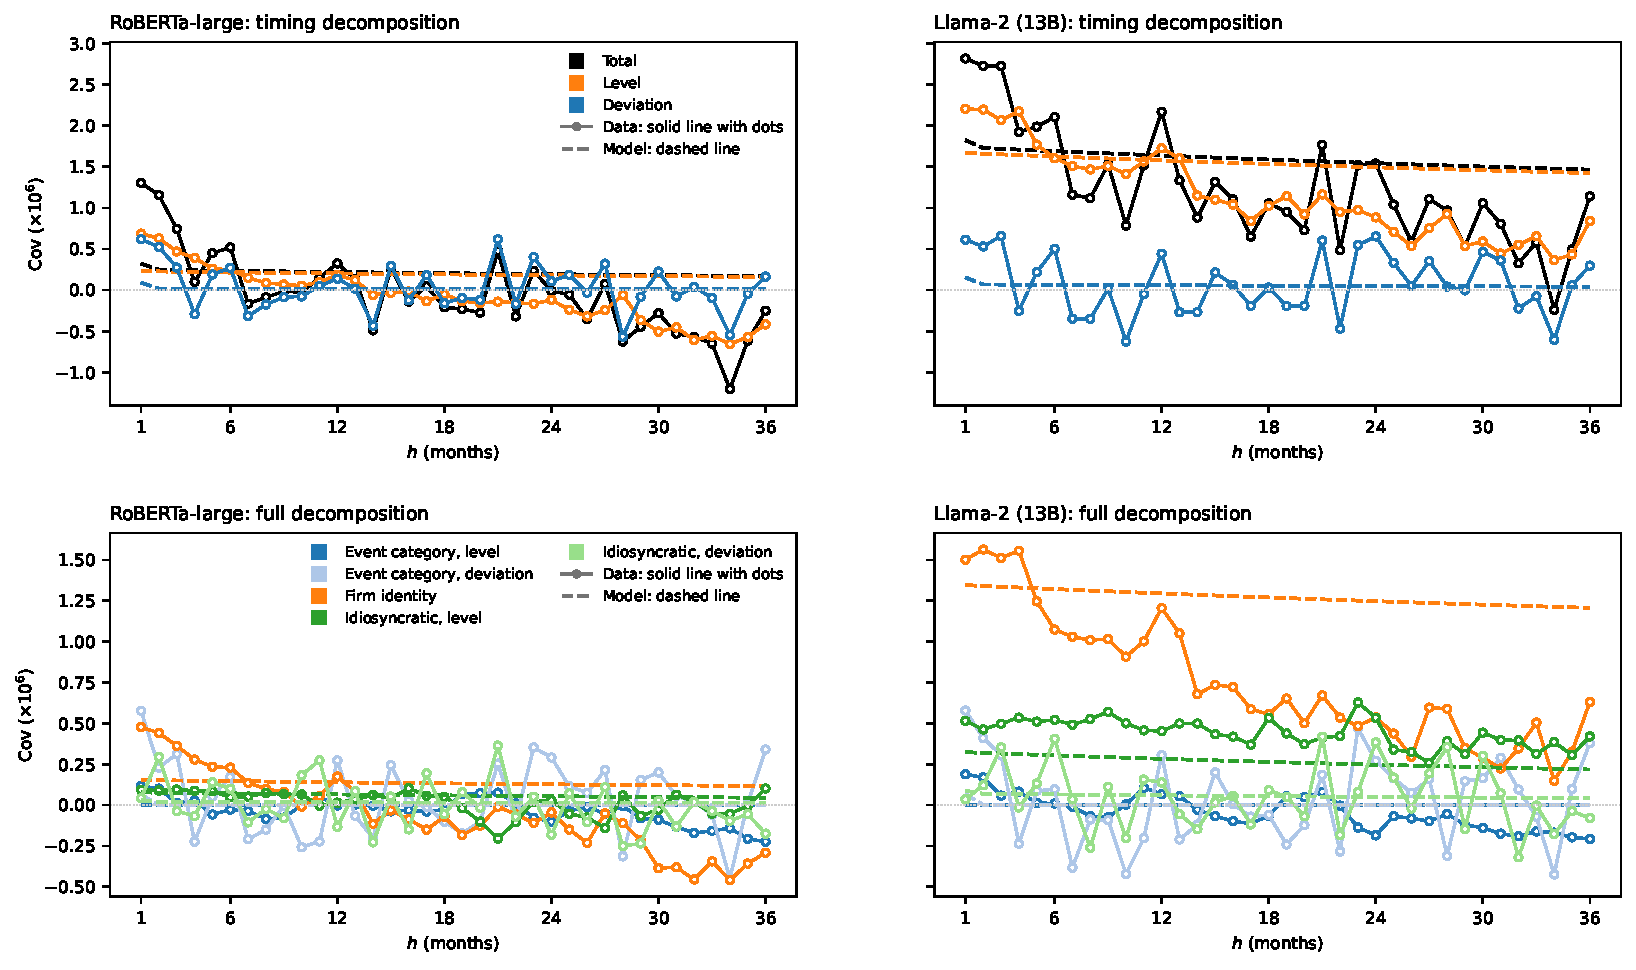
\includegraphics[width=\linewidth]{cal_fig2b.pdf}
\label{fig:pf2b}
\begin{minipage}{\linewidth}\footnotesize
This figure reports covariances of headline-weighted monthly averages of daily forecasts with returns $h$ months after the signal month. Columns show RoBERTa-large and Llama-2 (13B), with the timing decomposition (total, historical level, deviation) in the upper panels and the full decomposition ($C_L$, $C_D$, $F$, $I_L$, $I_D$) in the lower panels. Data are solid lines with dots and model values are dashed lines. These covariances are not calibration targets.
\end{minipage}
\end{figure}

The monthly projection forecast is a ridge forecast fitted to next-month returns on monthly average embeddings. In the model, the deviation's persistent information comes from the state's change relative to its historical level, with the coverage adjustments in \eqref{eq:D37}. The deviation accounts for 7.9\% of month-one predictive covariance for RoBERTa and 4.7\% for Llama-2, against 77.6\% and 55.6\% in the data. Figure~\ref{fig:pf2c} scales the model's total covariance to match the data at month one, leaving component shares and the horizon profile determined by the model.

\begin{figure}[!htbp]
\centering
\caption{Monthly Projection Forecast Covariances by Component and Horizon}
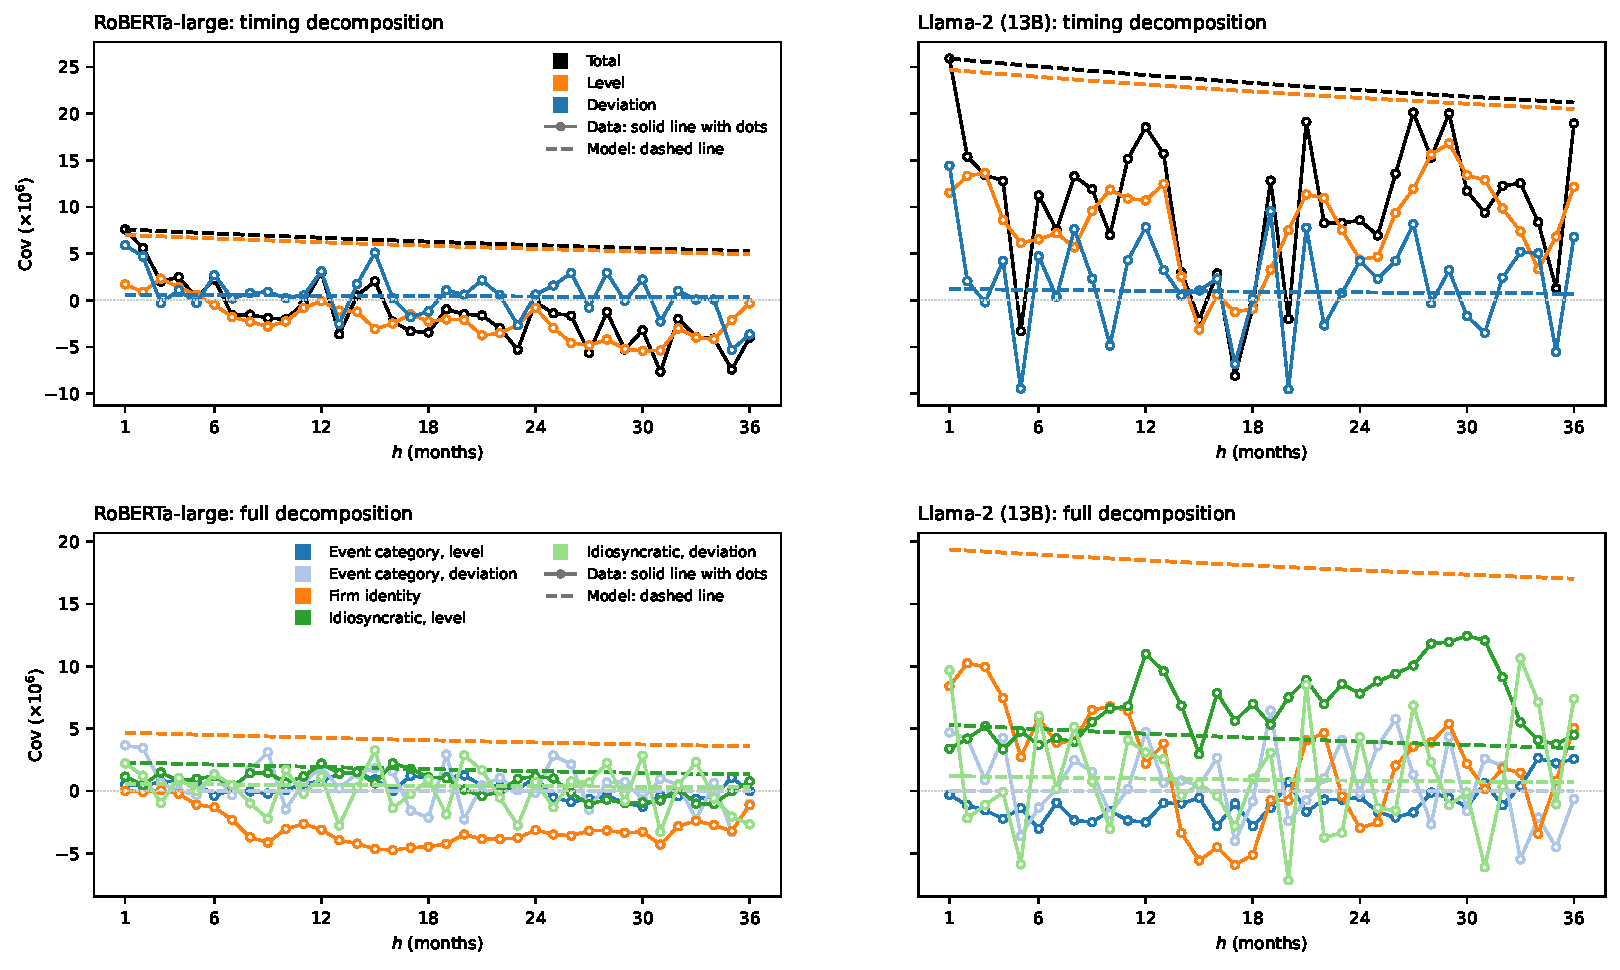
\includegraphics[width=\linewidth]{cal_fig2c.pdf}
\label{fig:pf2c}
\begin{minipage}{\linewidth}\footnotesize
This figure reports monthly projection forecast covariances with returns $h$ months after the signal month. Columns show RoBERTa-large and Llama-2 (13B), with the timing decomposition (total, historical level, deviation) in the upper panels and the full decomposition ($C_L$, $C_D$, $F$, $I_L$, $I_D$) in the lower panels. Data are solid lines with dots and model values are dashed lines. Model total covariance is scaled to match the data at month one.
\end{minipage}
\end{figure}

The residualized-embedding strategy also places more of its first-month return outside the historical level than the model implies. In the model, that return is $\Upsilon$ times the sum of \eqref{eq:D10} and \eqref{eq:D35} to \eqref{eq:D37}. The model places 92\% and 95\% of the return in the historical level for RoBERTa and Llama-2, against 51\% and 76\% in the data (Table~\ref{tab:tab13}). The category level, the category deviation, and the idiosyncratic deviation predict first-month returns well beyond the model. The category level alone carries about 15\% of RoBERTa's first-month return and 4\% of Llama-2's (Table 8 of the paper).

The category deviation accounts for 33\% of the first-month MSRR strategy return for RoBERTa and 16\% for Llama-2, against 0.1\% and 0.05\% in the model.
At month 12, its component return, after scaling the full strategy to 10\% annual volatility, is 4.06\% a year for RoBERTa and 1.77\% for Llama-2, against a negligible model return.
Part of the difference comes from the model's single drift speed. In the data, drift lasts about 20 trading days among micro stocks (below the 20th NYSE size percentile), which carry most of the category deviation's monthly predictability.
Another part reflects the horizon dependence of the MSRR weights (Section~\ref{sec:calibration}).

\subsection{Monthly Horizons}

Persistent firm information sustains the historical level's predictability at long horizons. The permanent state does not decay, and the evolving state has a calibrated half-life of 39 months. Figure~\ref{fig:pf3} compares component returns using the original MSRR coefficients at every horizon.

At the horizon-specific volatility scales in Figure~\ref{fig:pf3}, the historical level's return falls between months 1 and 36 by 21\% in the model and 42\% in the data for RoBERTa, and by 35\% and 55\% for Llama-2.
At month one, model firm-identity returns are 59\% and 85\% of the data's for RoBERTa and Llama-2.
For Llama-2, the model's idiosyncratic level is smaller than the data's, because one state loading scales both $F$ and $I_L$ while Llama-2's memory sits almost entirely in $F$.

\begin{figure}[!htbp]
\centering
\caption{Residualized-Embedding MSRR Strategy Component Returns by Monthly Horizon}
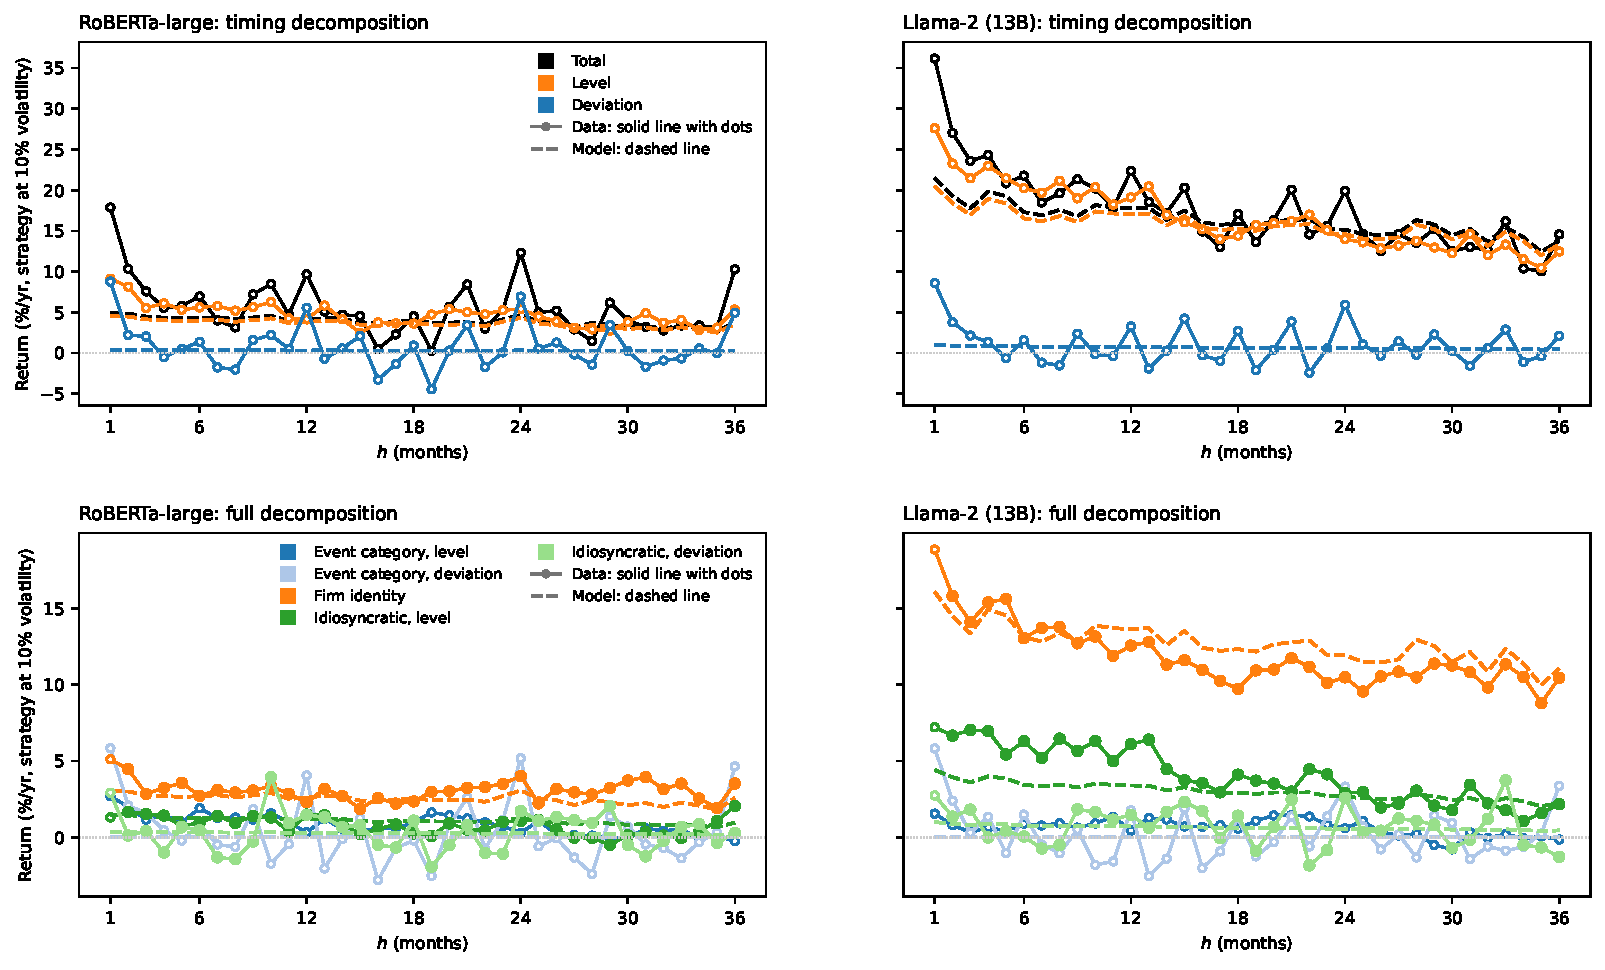
\includegraphics[width=\linewidth]{cal_fig3.pdf}
\label{fig:pf3}
\begin{minipage}{\linewidth}\footnotesize
This figure reports residualized-embedding MSRR strategy returns $h$ months after the signal month, holding MSRR coefficients fixed. Columns show RoBERTa-large and Llama-2 (13B), with the timing decomposition (total, historical level, deviation) in the upper panels and the full decomposition ($C_L$, $C_D$, $F$, $I_L$, $I_D$) in the lower panels. Data are solid lines with dots, targeted horizons have filled markers, and model values are dashed lines. At each horizon, the empirical strategy is scaled to 10\% annual volatility, and the same factor scales model component returns.
\end{minipage}
\end{figure}

The historical level lagged 36 months provides another check on persistence (Section~\ref{sec:lookahead}). Without memory, the model's lagged-level Sharpe ratio is 0.62 times the current level's. With memory, the model ratios are 0.68 for RoBERTa and 0.76 for Llama-2, against 0.27 and 0.56 in the data. ChronoGPT, which remembers none of the sample's cash-flow news, has a model ratio of 0.62 against 0.28 in the data. RoBERTa's and ChronoGPT's firm information therefore decays faster than the model's common persistence implies.

For the MSRR strategy fitted to the historical level, memory accounts for 47\% of Llama-2's model first-month mean return and 24\% of RoBERTa's, averaged over the strategies' signal months, including those after each encoder's pretraining cutoff (Table~\ref{tab:D2}). These shares differ from the memory shares in Table~\ref{tab:tab12}, which measure memory's shares of daily predictive covariance before January 2023 for Llama-2 and before January 2020 for RoBERTa. For the strategy fitted to the historical level 36 months earlier, memory's share rises to 66\% for Llama-2 and 40\% for RoBERTa, because lagging reduces the state contribution relative to memory by the square of \eqref{eq:D31}.

\subsection{Relative IC Ratios across the Cutoffs}

Across January 2023, Llama-2's forecast components all become more dispersed relative to RoBERTa's in similar proportions, as a change in Llama-2's forecast scale would make them. Table~\ref{tab:tab12} reports relative dispersion ratios between 1.27 and 1.38. For the category deviation, which carries no memory, the relative dispersion ratio is 1.27, while the relative IC ratio is 1.10. We therefore target relative IC ratios, which remove the forecast scale. The data use period-mean rank ICs.

\begin{table}[htbp]
\centering
\caption{Relative IC Ratios across the Pretraining Cutoffs}
\label{tab:tab12}
\begin{minipage}{\linewidth}\footnotesize
This table reports, by component $j$ of the daily ridge forecast, data and model values of the relative IC ratios $\mathrm{RIC}_j$ in \eqref{eq:D28}, Llama-2 relative to RoBERTa across January 2023, and $\mathrm{RIC}_j^*$ in \eqref{eq:D29}, RoBERTa relative to Llama-2 across January 2020 with dates through September 2022, with mean daily rank ICs with next open-to-open returns on common trading days. Each ratio divides one encoder's ratio of its later to its earlier mean IC by the same ratio for the other encoder. The historical level is the mean of the firm's monthly average forecast over its news months in the preceding 12 months; the deviation is the remainder. The dispersion ratio replaces each IC with the component's mean cross-sectional standard deviation. Memory share is the percentage of the split encoder's pre-split predictive covariance attributable to memory, $1-\omega_j^o$. Intervals come from a moving-block bootstrap with 40-trading-day blocks drawn separately before and after the split. Targeted marks the calibration targets.
\end{minipage}
\medskip

{\footnotesize
\begin{adjustbox}{max width=\linewidth}
\begin{tabular}{lcccccc}
\toprule
 & & \multicolumn{3}{c}{Data} & \multicolumn{2}{c}{Model} \\
\cmidrule(lr){3-5}\cmidrule(lr){6-7}
Component & Targeted & IC ratio & 90\% interval & Dispersion ratio & IC ratio & Memory share (\%) \\
\midrule
\multicolumn{7}{@{}l}{\textit{Llama-2 across January 2023, relative to RoBERTa}} \\
Firm identity $F$ & Yes & 0.32 & [0.13, 0.61] & 1.37 & 0.33 & 70 \\
Historical level $E_L$ & Yes & 0.36 & [0.21, 0.68] & 1.30 & 0.41 & 62 \\
Idiosyncratic level $I_L$ & No & 1.08 & [$-$3.19, 9.33] & 1.38 & 0.78 & 23 \\
Deviation $E_D$ & No & 1.23 & [1.03, 1.36] & 1.38 & 1.00 & 0 \\
Category deviation $C_D$ & No & 1.10 & [1.02, 1.16] & 1.27 & 1.00 & 0 \\
\midrule
\multicolumn{7}{@{}l}{\textit{RoBERTa across January 2020, relative to Llama-2}} \\
Firm identity $F$ & Yes & 1.18 & [$-$2.01, 5.08] & 0.95 & 0.89 & 11 \\
Historical level $E_L$ & Yes & 1.20 & [$-$0.27, 2.42] & 0.94 & 0.92 & 8 \\
Idiosyncratic level $I_L$ & No & 0.18 & [$-$3.96, 5.17] & 0.88 & 0.98 & 2 \\
Deviation $E_D$ & No & 0.99 & [0.85, 1.22] & 0.89 & 1.00 & 0 \\
Category deviation $C_D$ & No & 0.95 & [0.90, 1.05] & 0.91 & 1.00 & 0 \\
\bottomrule
\end{tabular}
\end{adjustbox}
}
\end{table}

Figure~\ref{fig:cutoff} in Section~\ref{sec:lookahead} shows the historical level's relative IC ratio across January 2023 by trading-day horizon. Its 90\% intervals exclude one at horizons of one to three trading days and include it at five and ten.

In the model, memory accounts for 70\% of Llama-2's covariance of firm identity before 2023 and 62\% of the historical level's. The model's relative IC ratios, 0.33 and 0.41 against 0.32 and 0.36 in the data, lie above one minus these shares because RoBERTa also loses memory across January 2023.

For RoBERTa's own comparison across January 2020, the memory loading $\eta=0.12$ gives model ratios of 0.89 for firm identity and 0.92 for the historical level, against 1.18 and 1.20 in the data. Memory accounts for 11\% and 8\% of its corresponding pre-split covariances. The data intervals are wide and include both one and the model ratios.

The deviation carries almost no memory, and its relative IC ratio in the model is approximately one. Across January 2023, the category deviation's and the overall deviation's data IC ratios lie 10\% and 23\% above one. A departure from the common-change assumption of the same sign in firm identity and the historical level would understate their memory.

In the model, memory is lost only when return dates pass the encoder's cutoff. It therefore does not explain why Llama-2's historical-level advantage over RoBERTa largely disappears from 2021, before its September 2022 cutoff (Figure 6 of the paper). The January 2023 split places 2021--2022 in the earlier period, which lowers Llama-2's earlier mean IC and thus the measured relative decline.

\section{Extensions of the Framework}\label{sec:extensions}

\paragraph{News arrival.}
For a firm with news in only some of the preceding twelve months, the historical level averages those months equally. If news arrival is independent of the state, the historical level's share of the evolving state's predictive covariance is the average of $\rho_m^\ell$ over its news months, where $\ell$ counts months before the signal month. News timing therefore changes the effective historical averaging weight.

\paragraph{Event categories.}
We can allow announcement responses and drift speeds to vary across event categories and firms. Slower drift among micro stocks (Section~\ref{sec:modeldata}) can leave more drift in the first month than the common response in Section~\ref{sec:param}. Allowing categories to depend on past news or the firm state would also let the category level predict returns through persistent differences in firms' category mixes. These extensions address event dynamics. The horizon dependence of MSRR weights discussed in Section~\ref{sec:calibration} provides a separate reason why the allocation of predictive content changes across horizons.

\paragraph{The firm state.}
We can let embeddings measure several firm-state components with different persistence. Encoder-specific loadings on these components would allow RoBERTa's and ChronoGPT's firm information to decay faster than Llama-2's, as in Section~\ref{sec:modeldata}. Changing a scalar loading on the same evolving state changes the magnitude of its predictive covariance, but not its decay rate.

\paragraph{Firm histories and memory.}
Memory in Section~\ref{sec:lookahead} covers every trading day in the window, whether or not the firm has published news. News histories instead determine how the decomposition allocates persistent firm information across $F$, $I_L$, and $I_D$, as described in Section~\ref{sec:calibration}. We can extend the model by allowing the memory loading to vary across firms. Holding the memory window and other sources of predictability fixed, a larger loading raises memory's contribution to predictive covariance. Table 11 of the paper reports Llama-2's relative historical-level IC ratios across January 2023 of 0.10 for big firms, against 0.26 for micro firms, and 0.16 for firms with high news intensity, against 0.47 for firms with low news intensity. These patterns are consistent with differences in memory shares across firms.

\paragraph{Estimation.}
Ridge shrinkage varies across predictive directions. A single monthly strategy scale $\Upsilon$ therefore approximates the allocation of MSRR strategy returns across components and horizons. Modeling this shrinkage explicitly, together with horizon-specific return projections, would allow the weights on event and state information to differ across forecast horizons. Same-day return residuals can also be correlated across firms. Such dependence can raise coefficient-estimation variance and make Proposition~\ref{prop:D1} understate estimation noise.

\section*{References}
\begin{enumerate}[label={[\arabic*]},leftmargin=*]

\item Altonji, J.\,G.\ and L.\,M.\ Segal (1996). Small-Sample Bias in GMM Estimation of Covariance Structures.
\emph{Journal of Business \& Economic Statistics} 14, 353--366.



\item Banerjee, S., B.\ Breon-Drish and J.\ Engelberg (2020). Discussion of ``Disclosure Processing Costs, Investors' Information Choice, and Equity Market Outcomes: A Review.''
\emph{Journal of Accounting and Economics} 70, 101337.

\item Campbell, J.\,Y.\ (1991). A Variance Decomposition for Stock Returns.
\emph{Economic Journal} 101, 157--179.

\item Campbell, J.\,Y.\ and R.\,J.\ Shiller (1988). The Dividend-Price Ratio and Expectations of Future Dividends and Discount Factors.
\emph{Review of Financial Studies} 1, 195--228.

\item Chen, Y., B.\,T.\ Kelly and D.\ Xiu (2026). Expected Returns and Large Language Models.
Working paper, SSRN 4416687.

\item Crane, L.\,D., A.\ Karra and P.\,E.\ Soto (2025). Total Recall? Evaluating the Macroeconomic Knowledge of Large Language Models.
Finance and Economics Discussion Series 2025-044, Board of Governors of the Federal Reserve System.

\item Didisheim, A., B.\,T.\ Kelly, M.\ Pourmohammadi and H.\ Tian (2026). The Inefficient Pricing of News.
NBER Working Paper 35093.

\item Gao, Z., W.\ Jiang and Y.\ Yan (2025). Detecting Lookahead Bias in LLM Forecasts.
arXiv:2512.23847.

\item He, S., L.\ Lv, A.\ Manela and J.\ Wu (2026). Chronologically Consistent Large Language Models.
\emph{Journal of Financial Economics} 185, 104374.

\item Jensen, T.\,I., B.\ Kelly and L.\,H.\ Pedersen (2023). Is There a Replication Crisis in Finance?
\emph{Journal of Finance} 78, 2465--2518.



\item Kelly, B.\,T., S.\ Malamud, J.\ Schwab and T.\,A.\ Xu (2026). Scaling Point-in-Time Language Models.
NBER Working Paper 35247.



\item Lopez-Lira, A., Y.\ Tang and M.\ Zhu (2025). The Memorization Problem: Can We Trust LLMs' Economic Forecasts?
arXiv:2504.14765.

\item Sarkar, S.\,K.\ and K.\ Vafa (2024). Lookahead Bias in Pretrained Language Models.
Working paper, SSRN 4754678.



\item Touvron, H., L.\ Martin, K.\ Stone et al.\ (2023). Llama 2: Open Foundation and Fine-Tuned Chat Models.
arXiv:2307.09288.

\item Vuolteenaho, T.\ (2002). What Drives Firm-Level Stock Returns?
\emph{Journal of Finance} 57, 233--264.

\end{enumerate}

\end{document}
